\documentclass[11pt,bibliography=totocnumbered]{scrartcl}
\usepackage[usenames,dvipsnames]{xcolor}
\usepackage[utf8]{inputenc}
\usepackage[T1]{fontenc}
\usepackage{fontspec-luatex}
\usepackage{amsmath,amssymb,amstext}
\usepackage{graphicx}
\usepackage[automark]{scrpage2}
\usepackage{url}
\usepackage[style=numeric-verb,backend=bibtex8,sorting=none, maxbibnames=99]{biblatex}
\usepackage[nottoc,numbib,notlof]{tocbibind}
\usepackage[ngerman]{babel}
\usepackage{titlesec}
\usepackage{tocloft}
\usepackage[bottom=1.5in]{geometry}
\usepackage{tikz}
\usepackage{pgfplots}
\usepackage[colorlinks=true,urlcolor=blue,linkcolor=Sepia,citecolor=Sepia,unicode,breaklinks=true,backref=true]{hyperref}
\usepackage[onehalfspacing]{setspace}
\usepackage{float}
\usepackage[parfill]{parskip}
\usepackage[utf8]{inputenc}
\usepackage{listings}
\usepackage{listings}
\usepackage{amsmath}
\usepackage{mathtools}
\usepackage{colortbl}
\usepackage{xpatch}
\usepackage{hhline}
\usepackage[xindy, nopostdot, nonumberlist]{glossaries}

\newcommand{\listequationsname}{Formelverzeichnis}
\newlistof{myequations}{equ}{\listequationsname}
\newcommand{\myequations}[1]{%
\addcontentsline{equ}{myequations}{\protect\numberline{\theequation}#1}}
\addtolength{\cftmyequationsnumwidth}{12pt}

\colorlet{punct}{red!60!black}
\definecolor{background}{HTML}{EEEEEE}
\definecolor{delim}{RGB}{20,105,176}
\colorlet{numb}{magenta!60!black}

\definecolor{maroon}{cmyk}{0, 0.87, 0.68, 0.32}
\definecolor{halfgray}{gray}{0.55}
\definecolor{ipython_frame}{RGB}{207, 207, 207}
\definecolor{ipython_bg}{RGB}{247, 247, 247}
\definecolor{ipython_red}{RGB}{186, 33, 33}
\definecolor{ipython_green}{RGB}{0, 128, 0}
\definecolor{ipython_cyan}{RGB}{64, 128, 128}
\definecolor{ipython_purple}{RGB}{170, 34, 255}

\definecolor{green_tp}{RGB}{122, 255, 140}
\definecolor{green_tn}{RGB}{214, 255, 220}
\definecolor{red_fp}{RGB}{255, 176, 176}
\definecolor{red_fn}{RGB}{255, 210, 171}

\lstset{
	breaklines=true,
	extendedchars=true,
	literate=
	{á}{{\'a}}1 {é}{{\'e}}1 {í}{{\'i}}1 {ó}{{\'o}}1 {ú}{{\'u}}1
	{Á}{{\'A}}1 {É}{{\'E}}1 {Í}{{\'I}}1 {Ó}{{\'O}}1 {Ú}{{\'U}}1
	{à}{{\`a}}1 {è}{{\`e}}1 {ì}{{\`i}}1 {ò}{{\`o}}1 {ù}{{\`u}}1
	{À}{{\`A}}1 {È}{{\'E}}1 {Ì}{{\`I}}1 {Ò}{{\`O}}1 {Ù}{{\`U}}1
	{ä}{{\"a}}1 {ë}{{\"e}}1 {ï}{{\"i}}1 {ö}{{\"o}}1 {ü}{{\"u}}1
	{Ä}{{\"A}}1 {Ë}{{\"E}}1 {Ï}{{\"I}}1 {Ö}{{\"O}}1 {Ü}{{\"U}}1
	{â}{{\^a}}1 {ê}{{\^e}}1 {î}{{\^i}}1 {ô}{{\^o}}1 {û}{{\^u}}1
	{Â}{{\^A}}1 {Ê}{{\^E}}1 {Î}{{\^I}}1 {Ô}{{\^O}}1 {Û}{{\^U}}1
	{œ}{{\oe}}1 {Œ}{{\OE}}1 {æ}{{\ae}}1 {Æ}{{\AE}}1 {ß}{{\ss}}1
	{ç}{{\c c}}1 {Ç}{{\c C}}1 {ø}{{\o}}1 {å}{{\r a}}1 {Å}{{\r A}}1
	{€}{{\EUR}}1 {£}{{\pounds}}1
}

\lstdefinelanguage{pythoninline}{
	morekeywords={access,and,break,class,continue,def,del,elif,else,except,exec,finally,for,from,global,if,import,in,is,lambda,not,or,pass,print,raise,return,try,while},
	morekeywords=[2]{abs,all,any,basestring,bin,bool,bytearray,callable,chr,classmethod,cmp,compile,complex,delattr,dict,dir,divmod,enumerate,eval,execfile,filter,float,format,frozenset,getattr,globals,hasattr,hash,help,hex,id,input,int,isinstance,issubclass,iter,len,list,locals,long,map,max,memoryview,min,next,object,oct,open,ord,pow,property,range,raw_input,reduce,reload,repr,reversed,round,set,setattr,slice,sorted,staticmethod,str,sum,super,tuple,type,unichr,unicode,vars,xrange,zip,apply,buffer,coerce,intern},
	sensitive=true,
	morecomment=[l]\#,
	morestring=[b]',
	morestring=[b]",
	morestring=[s]{'''}{'''},
	morestring=[s]{"""}{"""},
	morestring=[s]{r'}{'},
	morestring=[s]{r"}{"},
	morestring=[s]{r'''}{'''},
	morestring=[s]{r"""}{"""},
	morestring=[s]{u'}{'},
	morestring=[s]{u"}{"},
	morestring=[s]{u'''}{'''},
	morestring=[s]{u"""}{"""},
	% {replace}{replacement}{lenght of replace}
	% *{-}{-}{1} will not replace in comments and so on
	literate=
	{á}{{\'a}}1 {é}{{\'e}}1 {í}{{\'i}}1 {ó}{{\'o}}1 {ú}{{\'u}}1
	{Á}{{\'A}}1 {É}{{\'E}}1 {Í}{{\'I}}1 {Ó}{{\'O}}1 {Ú}{{\'U}}1
	{à}{{\`a}}1 {è}{{\`e}}1 {ì}{{\`i}}1 {ò}{{\`o}}1 {ù}{{\`u}}1
	{À}{{\`A}}1 {È}{{\'E}}1 {Ì}{{\`I}}1 {Ò}{{\`O}}1 {Ù}{{\`U}}1
	{ä}{{\"a}}1 {ë}{{\"e}}1 {ï}{{\"i}}1 {ö}{{\"o}}1 {ü}{{\"u}}1
	{Ä}{{\"A}}1 {Ë}{{\"E}}1 {Ï}{{\"I}}1 {Ö}{{\"O}}1 {Ü}{{\"U}}1
	{â}{{\^a}}1 {ê}{{\^e}}1 {î}{{\^i}}1 {ô}{{\^o}}1 {û}{{\^u}}1
	{Â}{{\^A}}1 {Ê}{{\^E}}1 {Î}{{\^I}}1 {Ô}{{\^O}}1 {Û}{{\^U}}1
	{œ}{{\oe}}1 {Œ}{{\OE}}1 {æ}{{\ae}}1 {Æ}{{\AE}}1 {ß}{{\ss}}1
	{ç}{{\c c}}1 {Ç}{{\c C}}1 {ø}{{\o}}1 {å}{{\r a}}1 {Å}{{\r A}}1
	{€}{{\EUR}}1 {£}{{\pounds}}1
	%
	{^}{{{\color{ipython_purple}\^{}}}}1
	{=}{{{\color{ipython_purple}=}}}1
	%
	{+}{{{\color{ipython_purple}+}}}1
	{*}{{{\color{ipython_purple}$^\ast$}}}1
	{/}{{{\color{ipython_purple}/}}}1
	%
	{+=}{{{+=}}}1
	{-=}{{{-=}}}1
	{*=}{{{$^\ast$=}}}1
	{/=}{{{/=}}}1,
	literate=
	*{-}{{{\color{ipython_purple}-}}}1
	{?}{{{\color{ipython_purple}?}}}1,
	%
	identifierstyle=\color{black}\ttfamily,
	commentstyle=\color{ipython_cyan}\ttfamily,
	stringstyle=\color{ipython_red}\ttfamily,
	keepspaces=true,
	showspaces=false,
	showstringspaces=false,
	rulecolor=\color{ipython_frame},
	frame=single,
	frameround={t}{t}{t}{t},
	framexleftmargin=6mm,
	numbers=left,
	numberstyle=\tiny\color{halfgray},
	backgroundcolor=\color{ipython_bg},
	% extendedchars=true,
	basicstyle=\fontsize{13}{15}\selectfont\ttfamily,
	keywordstyle=\color{ipython_green}\ttfamily,
	tabsize=2
}

\lstdefinelanguage{python}{
	morekeywords={access,and,break,class,continue,def,del,elif,else,except,exec,finally,for,from,global,if,import,in,is,lambda,not,or,pass,print,raise,return,try,while},
	morekeywords=[2]{abs,all,any,basestring,bin,bool,bytearray,callable,chr,classmethod,cmp,compile,complex,delattr,dict,dir,divmod,enumerate,eval,execfile,filter,float,format,frozenset,getattr,globals,hasattr,hash,help,hex,id,input,int,isinstance,issubclass,iter,len,list,locals,long,map,max,memoryview,min,next,object,oct,open,ord,pow,property,range,raw_input,reduce,reload,repr,reversed,round,set,setattr,slice,sorted,staticmethod,str,sum,super,tuple,type,unichr,unicode,vars,xrange,zip,apply,buffer,coerce,intern},
	sensitive=true,
	morecomment=[l]\#,
	morestring=[b]',
	morestring=[b]",
	morestring=[s]{'''}{'''},
	morestring=[s]{"""}{"""},
	morestring=[s]{r'}{'},
	morestring=[s]{r"}{"},
	morestring=[s]{r'''}{'''},
	morestring=[s]{r"""}{"""},
	morestring=[s]{u'}{'},
	morestring=[s]{u"}{"},
	morestring=[s]{u'''}{'''},
	morestring=[s]{u"""}{"""},
	% {replace}{replacement}{lenght of replace}
	% *{-}{-}{1} will not replace in comments and so on
	literate=
	{á}{{\'a}}1 {é}{{\'e}}1 {í}{{\'i}}1 {ó}{{\'o}}1 {ú}{{\'u}}1
	{Á}{{\'A}}1 {É}{{\'E}}1 {Í}{{\'I}}1 {Ó}{{\'O}}1 {Ú}{{\'U}}1
	{à}{{\`a}}1 {è}{{\`e}}1 {ì}{{\`i}}1 {ò}{{\`o}}1 {ù}{{\`u}}1
	{À}{{\`A}}1 {È}{{\'E}}1 {Ì}{{\`I}}1 {Ò}{{\`O}}1 {Ù}{{\`U}}1
	{ä}{{\"a}}1 {ë}{{\"e}}1 {ï}{{\"i}}1 {ö}{{\"o}}1 {ü}{{\"u}}1
	{Ä}{{\"A}}1 {Ë}{{\"E}}1 {Ï}{{\"I}}1 {Ö}{{\"O}}1 {Ü}{{\"U}}1
	{â}{{\^a}}1 {ê}{{\^e}}1 {î}{{\^i}}1 {ô}{{\^o}}1 {û}{{\^u}}1
	{Â}{{\^A}}1 {Ê}{{\^E}}1 {Î}{{\^I}}1 {Ô}{{\^O}}1 {Û}{{\^U}}1
	{œ}{{\oe}}1 {Œ}{{\OE}}1 {æ}{{\ae}}1 {Æ}{{\AE}}1 {ß}{{\ss}}1
	{ç}{{\c c}}1 {Ç}{{\c C}}1 {ø}{{\o}}1 {å}{{\r a}}1 {Å}{{\r A}}1
	{€}{{\EUR}}1 {£}{{\pounds}}1
	%
	{^}{{{\color{ipython_purple}\^{}}}}1
	{=}{{{\color{ipython_purple}=}}}1
	%
	{+}{{{\color{ipython_purple}+}}}1
	{*}{{{\color{ipython_purple}$^\ast$}}}1
	{/}{{{\color{ipython_purple}/}}}1
	%
	{+=}{{{+=}}}1
	{-=}{{{-=}}}1
	{*=}{{{$^\ast$=}}}1
	{/=}{{{/=}}}1,
	literate=
	*{-}{{{\color{ipython_purple}-}}}1
	{?}{{{\color{ipython_purple}?}}}1,
	%
	identifierstyle=\color{black}\ttfamily,
	commentstyle=\color{ipython_cyan}\ttfamily,
	stringstyle=\color{ipython_red}\ttfamily,
	keepspaces=true,
	showspaces=false,
	showstringspaces=false,
	rulecolor=\color{ipython_frame},
	frame=single,
	frameround={t}{t}{t}{t},
	framexleftmargin=6mm,
	numbers=left,
	numberstyle=\tiny\color{halfgray},
	backgroundcolor=\color{ipython_bg},
	% extendedchars=true,
	basicstyle=\fontsize{10}{12}\selectfont\ttfamily,
	keywordstyle=\color{ipython_green}\ttfamily,
	tabsize=2
}

\lstdefinelanguage{json}{
	basicstyle=\normalfont\ttfamily,
	numbers=left,
	numberstyle=\scriptsize,
	stepnumber=1,
	numbersep=8pt,
	showstringspaces=false,
	breaklines=true,
	tabsize=2,
	frame=lines,
	backgroundcolor=\color{background},
	literate=
	*{0}{{{\color{numb}0}}}{1}
	{1}{{{\color{numb}1}}}{1}
	{2}{{{\color{numb}2}}}{1}
	{3}{{{\color{numb}3}}}{1}
	{4}{{{\color{numb}4}}}{1}
	{5}{{{\color{numb}5}}}{1}
	{6}{{{\color{numb}6}}}{1}
	{7}{{{\color{numb}7}}}{1}
	{8}{{{\color{numb}8}}}{1}
	{9}{{{\color{numb}9}}}{1}
	{:}{{{\color{punct}{:}}}}{1}
	{,}{{{\color{punct}{,}}}}{1}
	{\{}{{{\color{delim}{\{}}}}{1}
	{\}}{{{\color{delim}{\}}}}}{1}
	{[}{{{\color{delim}{[}}}}{1}
	{]}{{{\color{delim}{]}}}}{1},
}



\addbibresource{Quellen.bib}
\nocite{*}

\title{Automatische Analyse von Stimmmerkmalen zur Vorhersage von Persönlichkeitsprofilen mittels Künstlicher Intelligenz.}
\author{Sebastian Schmidt}
\date{\today{}, Iserlohn}

\renewcommand*\contentsname{Inhaltsverzeichnis}
\renewcommand\refname{Quellen}
\renewcommand{\thesection}{\arabic{section}.}
\renewcommand{\cftsecleader}{\cftdotfill{\cftdotsep}}
\renewcommand{\thesubsection}{\thesection\arabic{subsection}.}
\renewcommand{\thesubsubsection}{\thesubsection\arabic{subsubsection}.}
\renewcommand\cftsecafterpnum{\vskip10pt}

\renewcommand{\lstlistlistingname}{Listingverzeichnis}
\setlength{\cftfigindent}{0pt}
\makeatletter
\xpatchcmd\l@lstlisting{1.5em}{0em}{}{}
\makeatother

\titleformat{\paragraph}
{\normalfont\normalsize\bfseries}{\theparagraph}{1em}{}
\titlespacing*{\paragraph}
{0pt}{3.25ex plus 1ex minus .2ex}{1.5ex plus .2ex}
\titlespacing*{\subsubsection}
{0pt}{5mm}{3mm}

\begin{document} 
\KOMAoptions{fontsize=12pt}
\pagenumbering{gobble}
\setmainfont{Caladea}
\begin{titlepage}
	\centering
	
\includegraphics[width=0.45\textwidth]{fh-swf-logo}\par\vspace{1cm}
	{\scshape\Large Bachelorarbeit\par}
	\vspace{0.5cm}
	{\huge\bfseries Automatische Analyse von Stimmmerkmalen zur Vorhersage von Persönlichkeitsprofilen mittels Künstlicher Intelligenz\par}
	\vspace{1cm}
	{\Large\itshape Sebastian Schmidt\par}
	Matrikelnummer: 10053783\par
	E-Mail: schmidt.sebastian2@fh-swf.de\par
	\vspace{1cm}
	Erstprüfer: 
	Prof. Dr. Michael Rübsam\\ 
	\vspace{1mm}
	Zweitprüfer: 
	Prof. Dr. Christian Gawron
	\vfill
	
	% Bottom of the page
	{\large 25. Oktober 2019\par}
\end{titlepage}
\pagebreak
\paragraph{Eigenständigkeitserklärung}
Ich erkläre, dass ich die Arbeit selbständig angefertigt und nur die angegebenen Hilfsmittel benutzt habe. Alle Stellen, die dem Wortlaut oder dem Sinn nach anderen Werken, gegebenenfalls auch elektronischen Medien, entnommen sind, sind von mir durch Angabe der Quelle als Entlehnung kenntlich gemacht. Entlehnungen aus dem Internet sind durch Angabe der Quelle und des Zugriffsdatums belegt. Weiterhin habe ich die vorliegende 
Arbeit an keiner anderen Stelle zur Erlangung eines Abschlusses vorgelegt.

\vspace{50pt}
\noindent\rule{5cm}{.4pt}\hspace{4.8cm}\rule{5cm}{.4pt}\par
\noindent Datum, Ort \hspace{10.5cm} Unterschrift
\pagebreak
\tableofcontents
\pagebreak
\listoffigures
\lstlistoflistings
\pagebreak
\listofmyequations
\pagenumbering{arabic}
\pagestyle{scrheadings}
\clearscrheadfoot
\ohead[\pagemark]{\pagemark}
\ihead[]{\headmark}
\setcounter{equation}{0}
\pagebreak
\section{Einleitung}
\section{Eingrenzung}
\section{Theoretische Grundlagen}
In diesem Abschnitt sollen theoretische Grundlagen des Maschinellen Lernens vorgestellt werden. Es wird zunächst auf allgemeine Grundlagen eingegangen, um im folgenden auf die spezielleren Neuronalen Netze und Konvolutionellen Neuronale Netze einzugehen.
\subsection{Allgemeine Grundlagen des Maschinellen Lernens}
Maschinelles Lernen gibt einem Computer die Möglichkeit zu lernen ohne explizit von einem Entwickler für eine Aufgabe programmiert zu werden. Tom Mitchell beschreibt Maschinelles Lernen 1997 mit einem Computerprogramm das ohne Veränderungen des Programmcodes aus Erfahrungen E im Bezug auf eine Aufgabe T und ein Maß für die Leistung P lernt, indem seine Leistung P mit der Erfahrung E anwächst \cite[S. 4]{MACHINE_LEARNING}. Erfahrungen sammelt ein System, indem Daten mit speziellen Algorithmen betrachtet werden. Auf Basis dieser Daten erstellt der Algorithmus dann eine Strukturbeschreibung, welche auch als Modell bezeichnet wird \cite[S. 2]{DEEP_LEARNING}.
\\\\
In diesem Projekt wäre die Aufgabe das Klassifizieren von Gebärdensprache. Die Leistung des Modells würde durch die korrekte Klassifizierung beschrieben werden, welche idealerweise während des Trainingsvorgangs beim Anlernen von Datensätzen zu Gebärdensprache ansteigen sollte.
\subsubsection{Arten von Verfahren des Maschinellen Lernens}
Verfahren des Maschinellen Lernens werden in der Literatur häufig mittels verschiedener Kategorien in verschiedene Arten aufgeteilt. Auch wenn viele Arten von Verfahren in dieser Arbeit nicht betrachtet werden, ist es wichtig diese zu benennen, um ein passendes Verfahren auszuwählen. Es werden typischerweise drei Kategorien betrachtet, die Verfahren einteilen \cite[S.8-14]{MACHINE_LEARNING}\cite[S.2]{BA}. 
\\\\
Zunächst wird ein Verfahren danach eingeteilt, welche Informationen zu den Trainingsdaten anhand von Label nötig sind. Muss jeder Datenpunkt mit einem Label versehen sein, so handelt es sich um Überwachtes Lernen. Dem gegenüber steht das Unüberwachte Lernen, bei dem ein Algorithmus versucht Aussagen über mögliche Label aufgrund der Struktur der Daten zu treffen. Das Halbüberwachte Lernen kombiniert beide Eigenschaften und der Algorithmus versucht zunächst Label anzulernen, um im Folgenden autonom fortzufahren. Abschließend sei noch das Reinforcement Lernen zu nennen. Dieses bestraft und belohnt Aktionen auf eine vorher definierte Weise. Der Algorithmus versucht dann möglichst viele Belohnungen in möglichst wenig Zeit zu erhalten und gleichzeitig Bestrafungen zu verhindern \cite[S.8-14]{MACHINE_LEARNING}\cite[S.2]{BA}.
\\\\
Eine weitere Kategorie ist die Art wie ein Lernverfahren mit Daten versorgt werden muss. Beim Batch-Learning muss das Verfahren auf Basis eines kompletten Datensatzes trainiert und kann danach nicht mehr mit weiteren Daten verbessert werden. Es muss von Grund auf neu trainieren. Dem gegenüber steht das Online-Learning, welches nach und nach trainiert wird, und noch eine spätere Verfeinerung ermöglicht \cite[S.14-17]{MACHINE_LEARNING}\cite[S.2]{BA}.
\\\\
Mit einer weiteren Kategorie wird festgelegt wie ein Verfahren Daten verallgemeinert, um neue Aussagen treffen zu können. Mit modellbasierten Lernen wird anhand der Daten ein mathematisches Modell erstellt, welches versucht die Struktur der Daten korrekt zu beschreiben, um neue Vorhersagen treffen zu können. Instanzbasiertes Lernen vergleicht bei vorherzusagenden Daten die Merkmale mit bereits angelernten Datensätzen. Werden hier Ähnlichkeiten in den bereits erlernten Instanzen entdeckt, werden diese für eine neue Aussage genutzt \cite[S.14-17]{MACHINE_LEARNING}\cite[S.2]{BA}.
\\\\
Ebenfalls lassen sich Verfahren nach der Art des zu lösenden Problems einteilen. Bei der Klassifikation werden Daten anhand ihrer Label einer gewissen Klasse zugeordnet. Das Ziel ist es nun die Klasse von neuen Datensätzen korrekt vorherzusagen. Demgegenüber stehen Regressionsprobleme bei denen ein Label einen konkreten Wert angibt, welcher bei einem neuen Datensatz vom Modell korrekt vorhergesagt werden muss \cite[S.8-9]{MACHINE_LEARNING}\cite[S.2]{BA}.
\\\\
Bei dem in dieser Arbeit zu lösenden Problem handelt es sich um ein typisches Klassifikationsproblem des Überwachten Lernens. Ein Modell wird auf Basis von vorklassifizierten Daten, also typischerweise Datensätze mit Bildern von Händen die ein Zeichen in Gebärdensprache repräsentieren,  angelernt. Dieses soll dann im Folgenden weitere Bilder korrekt einem Zeichen in Gebärdensprache zuweisen können. Instanzbasiertes Lernen könnte bei Bilddaten zu Problemen führen. Da Bilder in der Regel relativ viele Daten beinhalten, könnte ein Merken der Beispiele zu sehr großen Modellen führen \cite[S.18]{MACHINE_LEARNING}. Aus diesem Grund sollte modellbasiertes Lernen vorgezogen werden. Es ist allerdings sowohl Batch-Learning als auch Online-Learning denkbar.
\subsubsection{Typische Probleme beim Maschinellen Lernen}
Beim Maschinellen Lernen können viele Probleme auftreten, die den Lernerfolg eines Modells behindern können. Um diesen entgegenwirken zu können, sollten typische Probleme vor dem Entwickeln eines Modells betrachtet werden.
\\\\
Schon bei einfachen Problemen ist eine ausreichende Datenmengen nötig, um Modelle antrainieren zu können. Abhängig von der Komplexität eines Problems und des genutzten Algorithmus, können Tausende bis Millionen von Datensätzen für einen Lernvorgang nötig sein \cite[S.23]{MACHINE_LEARNING}\cite[S.4]{BA}.
\\\\
Wurden Daten fehlerhaft gesammelt und repräsentieren nicht das Spektrum der möglichen Eingabe im Einsatz, so kann ein Modell keine korrekten Vorhersagen für den geplanten Einsatz treffen, da hier das Wertespektrum nicht das Gelernte repräsentiert. Auch eine ungünstige Verteilung von Klassen in den Daten, kann zu Probleme führen, besonders wenn dieser Fall mit unpassenden Qualitätsmaßen ausgewertet wird \cite[S.24-25]{MACHINE_LEARNING}\cite[S.4]{BA}.
\\\\
Minderwertige Daten erschweren ebenfalls den Lernvorgang. Dies kann sich durch verrauschte, fehlerhafte und fehlende Daten sowie Ausreißer äußern. Eine manuelle oder automatische Vorverarbeitung könnte dies verbessern. Sogar ein Auslassen bestimmter Merkmale kann sich als sinnvoll herausstellen. \cite[S.26]{MACHINE_LEARNING}\cite[S.3]{BA}. Hilft dies nicht ist ein Sammeln von neuen Datensätzen sinnvoll.
\\\\
Irrelevante oder schlecht gewählte Merkmale für das Antrainieren eines Datensatzes führen ebenfalls zu einem schlechteren oder gar keinem Lernerfolg. Für das Vorhersagen von Gebärdensprache, sollte zum Beispiel das Datum des vorherzusagenden Bildes keinen Einfluss haben. Wird diese Information im Trainingsvorgang trotzdem einbezogen, so ist mit einer schlechteren Performanz des Lernvorgangs zu rechnen \cite[S.26]{MACHINE_LEARNING}\cite[S.4]{BA}. 
\\\\
Overfitting tritt auf, wenn ein Modell für die Trainingsdaten zu komplex gewählt ist. Es führt dazu, dass ein Modell nicht korrekt verallgemeinert, sondern zufällige Variationen in den Trainingsdaten lernt. Es äußert sich in einer guten Performanz im Training, während diese in Tests nachlässt. Verhindern lässt sich dies im Modell durch eine Verringerung der Zahl der Parameter oder bestimmter Techniken, die dem Modell Restriktionen auflegen, der sogenannten Regularisierung. Außerdem lässt es sich durch Sammeln neuer, sowie der Verringerung von Rauschen in vorhandenen, Daten reduzieren \cite[S.27]{MACHINE_LEARNING}\cite[S.13]{BA}.
\begin{figure}[H] 
	\centering
	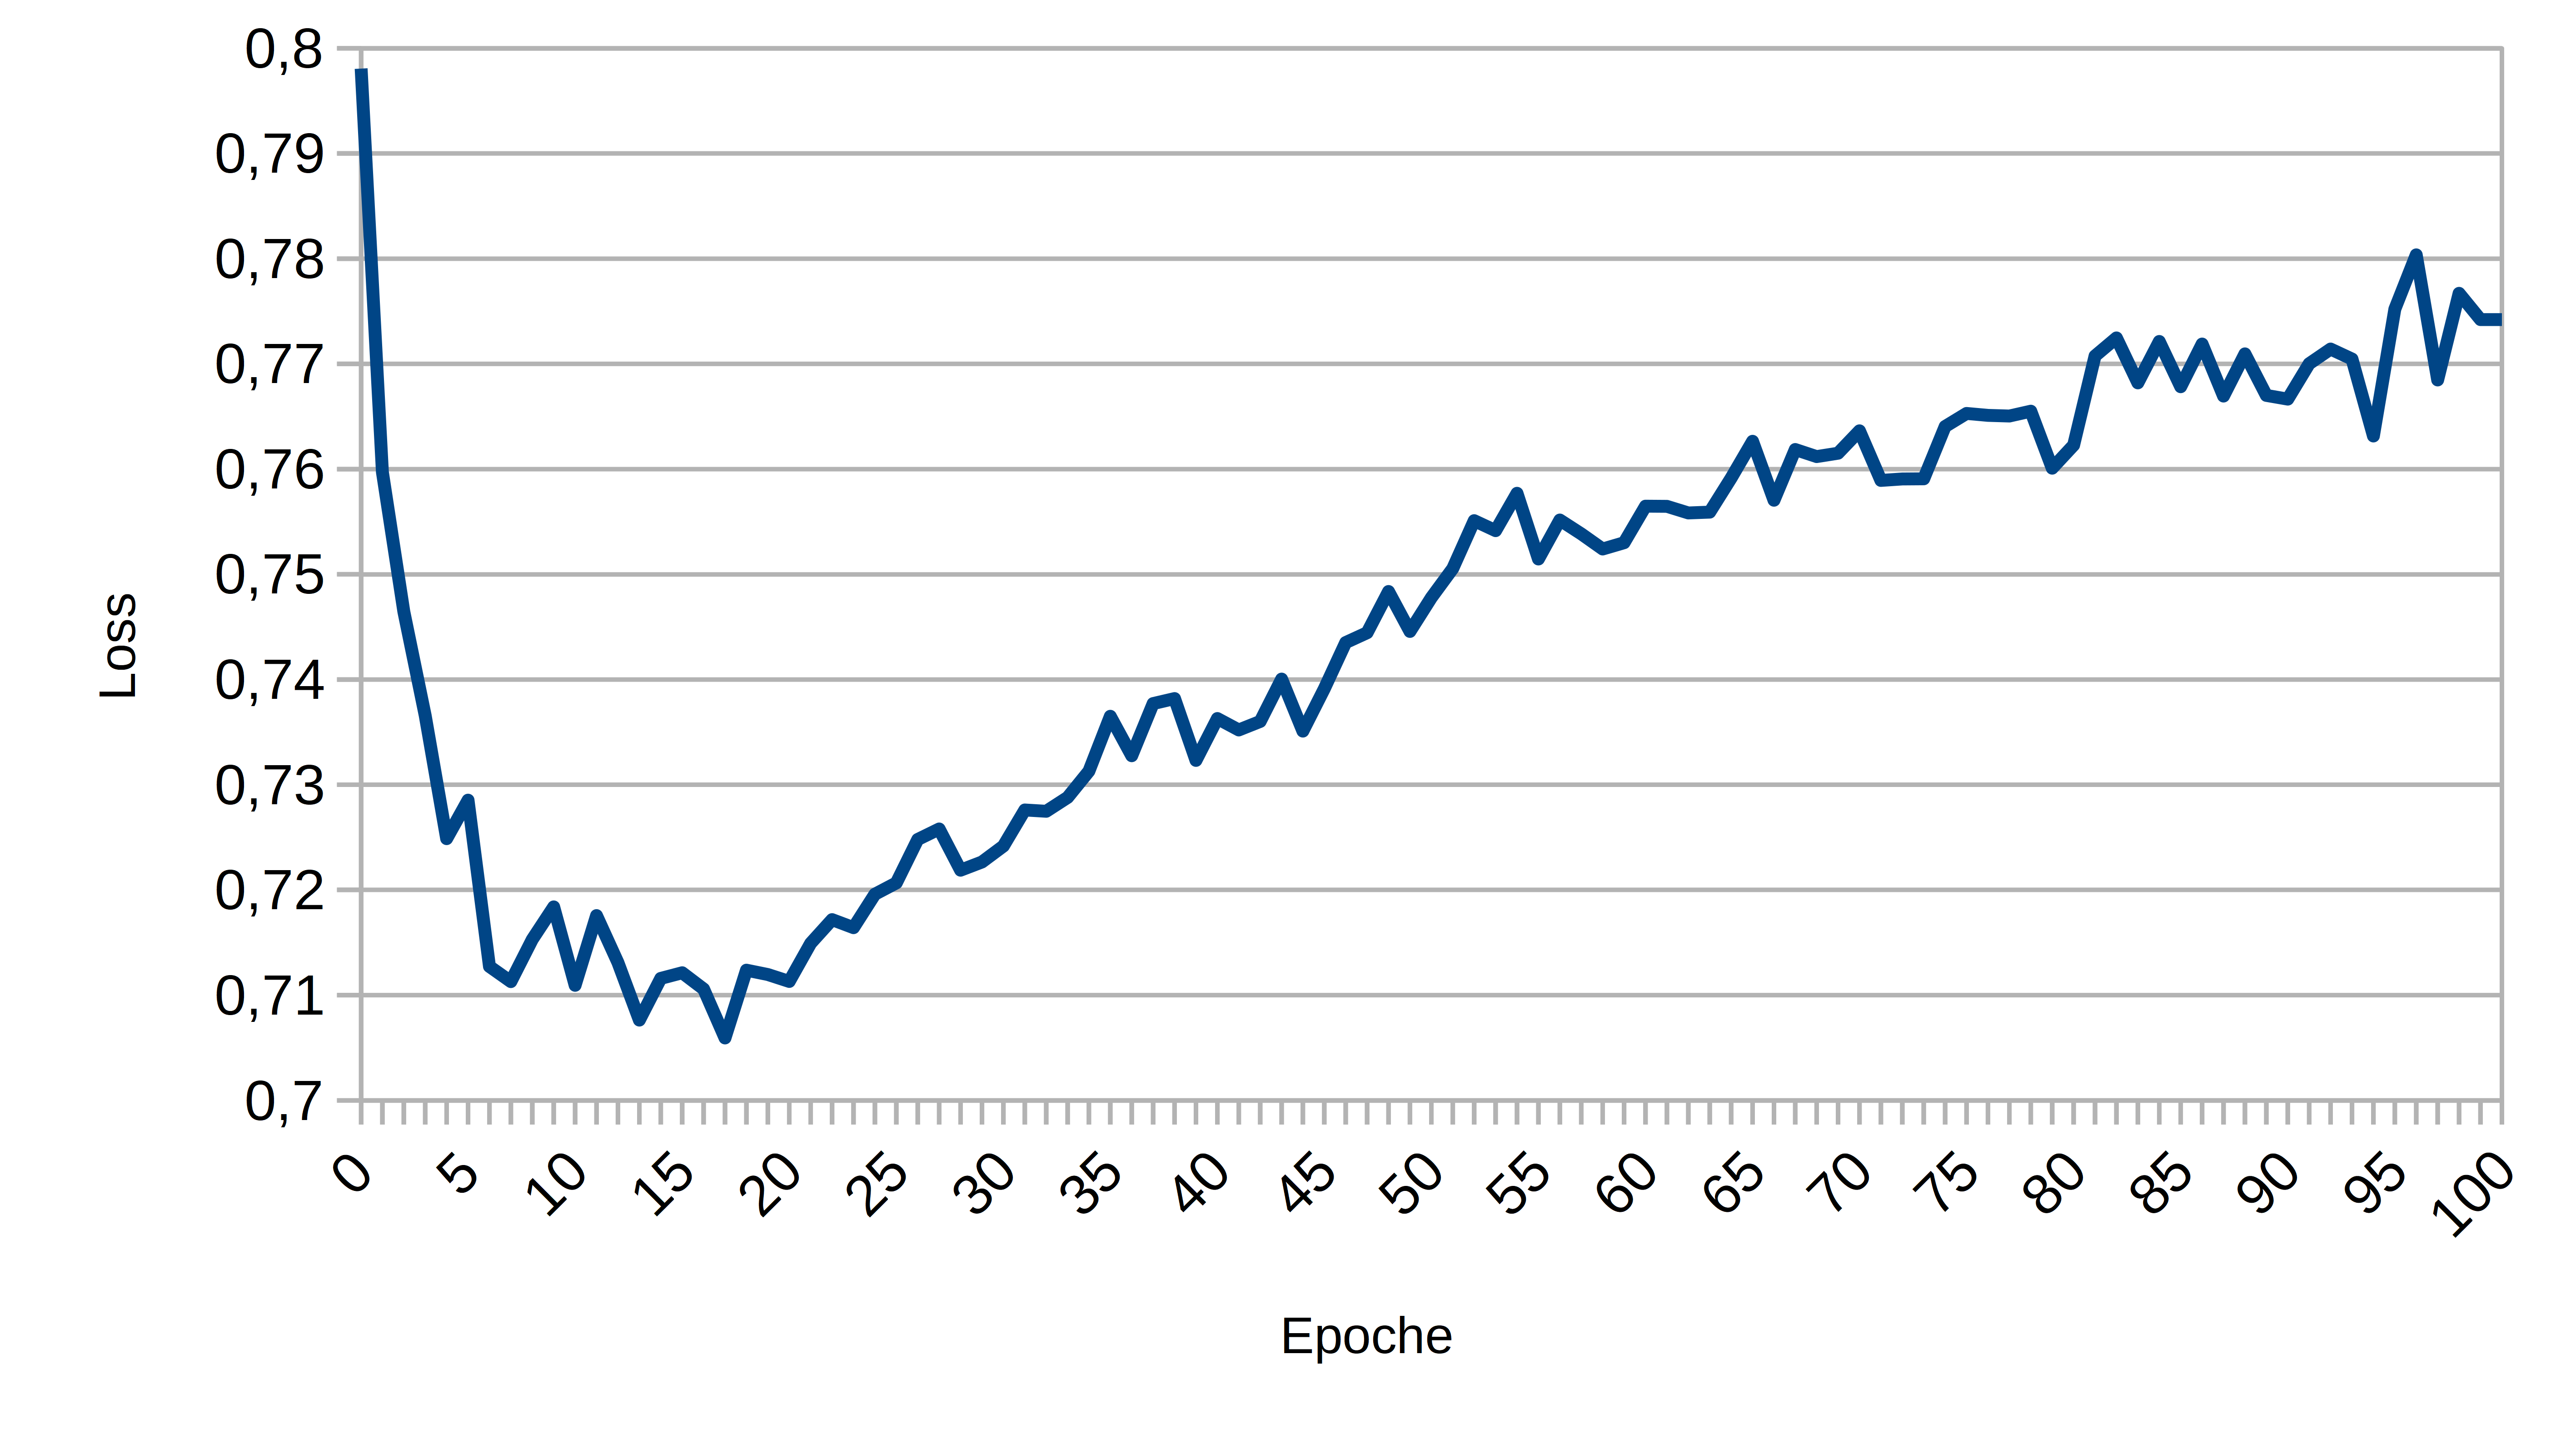
\includegraphics[width=1.0\textwidth]{mlp_5_loss}
	\caption[Overfitting in einem mehrschichtigen Neuronalen Netz]{Nach der 20. Epoche, tritt in diesem mehrschichtigen Neuronalen Netz ein Overfitting auf \cite[S.14]{BA}.}
	\label{fig:mlp_overfitting}
\end{figure}
Zuletzt sei das Underfitting genannt, welches dem Overfitting gegenübersteht. Ein Modell ist dabei zu einfach, um die Strukturen in den Trainingsdaten anzulernen. Modelle mit mehr Parametern, bessere Merkmale oder eine Verringerung der Regularisierung, reduzieren in der Regel ein Overfitting \cite[S.29]{MACHINE_LEARNING}\cite[S.14]{BA}.
\subsubsection{Datenvorverarbeitung für Bilddaten}
Wie im vorherigen Kapitel dargestellt, würden qualitativ unzureichende Daten zu einer schlechteren Performanz beim Anlernen eines Modells führen. Dies kann auch bei Bilddaten der Fall sein und sollte durch Vorverarbeitungsschritte verhindert werden. In dieser Sektion sollen einige typische Schritte der Bildvorverarbeitung dargestellt werden.
\\\\
Verrauschte Bilder können bei der Bilderkennung große Probleme darstellen. Ist ein Bild in keiner Weise rauschfrei, wurde gezeigt, dass Verfahren zum Entfernen von Rauschen eine positiven Effekt haben können \cite{RAUSCH}. Dieses Verfahren wurde im Praxisteil zwar, aufgrund des qualitativ hochwertigen Datensatzes, nicht genutzt, stellt aber für die Zukunft, besonders im Einsatz wo die Qualität der Bilddaten nicht immer gewährleistet ist, eine gute Methode zu einer möglichen Verbesserung dar.
\\\\
Ein weiterer Datenvorverarbeitungsschritt ist das Extrahieren von relevanten Bildausschnitten. Die meisten Datensätze für die Erkennung von Gebärdensprache, haben hier bereits die relevanten Ausschnitte vorverarbeitet, sodass nur noch die Hände zu sehen sind. Dies ist jedoch ein Problem für die Praxis, da ein Bild einer Webcam in der Regel mehr als nur die Hand beinhaltet. Es würde hier das Problem entstehen, dass die Daten in der Praxis nur wenig mit dem Angelernten übereinstimmen. Hier ist es sinnvoll den relevanten Teil eines Bildes zu extrahieren. Dazu wurde im Praxisteil ein Machine-Learning Framework names MediaPipe genutzt \cite{MEDIAPIPE}.
\\\\
Zuletzt müssen Bilder in der Regel vor der Nutzung skaliert werden. Ein Modell des Maschinellen Lernens erwartet in der Regel eine feste Eingabegröße. Dies gilt auch für Bilder, sodass als Beispiel das VGG19 Konvolutionelle Neuronale Netzwerk für Objekterkennung eine Eingabegröße von 224 x 224 Pixeln erwartet \cite[S.2]{SCALE}. Auch mit Blick auf die Laufzeit ergibt eine Skalierung von Bildern Sinn. Moderne Webcams erreichen schon häufig eine Auflösung von 1920 x 1080 Pixeln. Dies würde bei unskalierten und nicht extrahierten Bildinformationen zu einer Eingabegröße von 2. Millionen Parametern führen, was abhängig vom Modell zu sehr hohen Laufzeiten führen kann. Typische Algorithmen zum herunterskalieren von Bildern sind die Nächste-Nachbarn, Bilineare und Bikubische Interpolation \cite[S.2]{SCALE}.
\subsubsection{Qualitätsmaße}
Um die Leistung eines Modells korrekt bewerten zu können, müssen abhängig vom Ziel Qualitätsmaße eingeführt werden, die es möglich machen Modelle zu vergleichen. Dazu wird mit der Kreuzentropie ein typisches Qualitätsmaß für Klassifikationsprobleme eingeführt. Außerdem werden die Begriffe Konfusionsmatrix, Accuracy, Precision, Recall und F1-Score diskutiert.
\\\\
In praktisch allen Fällen können Algorithmen des Maschinellen Lernens nicht mit Klassenbezeichnungen in Form von Strings umgehen. Eine Menge von Klassenbezeichnungen wie \ensuremath{\{a, b, c \}} könnte nur schwierig direkt von Algorithmen als Label genutzt werden. Hier werden in der Regel zwei Möglichkeiten genutzt, um Bezeichnungen in nützlichere Label umzuwandeln. Diese wären:
\begin{itemize}
	\item Klassen-IDs: Die vorher angegebene Menge von Klassenbezeichnungen könnte in eine Menge von repräsentierenden IDs transformiert werden. So wird die Menge \ensuremath{\{a, b, c \}} in die IDs \ensuremath{\{0, 1, 2 \}} umgewandelt. Der Algorithmus muss bei der Klassifikation nun eine korrekte IDs vorhersagen, welche eine Klasse repräsentiert. Aufgrund der Arbeitsweise vieler Algorithmen nehmen diese allerdings an, dass IDs die näher beieinander liegen ähnlicher zueinander sind. Dies ist nicht für alle Problemstellungen ideal \cite[S.12]{BA}\cite[S.63]{MACHINE_LEARNING}.
	\item One-Hot-Kodierung: Bei diesem Verfahren wird für jede Klasse eine Zahl in einem Vektor reserviert. Eine vorliegende Klasse wird dann in der Regel mit einer 1 und der Rest der Elemente mit einer 0 markiert. Für die Beispielmenge \ensuremath{\{a, b, c \}} ergebe sich daher die Menge von Vektoren \ensuremath{\{\left(\begin{smallmatrix}1 & 0 & 0\end{smallmatrix}\right), \left(\begin{smallmatrix}0 & 1 & 0\end{smallmatrix}\right), \left(\begin{smallmatrix}0 & 0 & 1\end{smallmatrix}\right)\}}. Korrekt klassifiziert wurde nun, wenn der vorliegende Klasse mit der höchsten Vorhersagen markiert wird. Da in diesem Fall keine Beziehung zwischen den Klassen erkannt wird, ist dieses Darstellung auch ideal für die Problemstellung \cite[S.12]{BA}\cite[S.63]{MACHINE_LEARNING}.
\end{itemize}
Die bereits vorher erwähnte Kreuzentropie ist ein ideales Qualitätsmaß für Klassifikationsprobleme in One-Hot-Kodierung. Niedrige Vorhersagen bei der vorliegenden Klassen werden dabei abgestraft, während andere Vorhersagen ignoriert werden. Für einen Datensatz mit \ensuremath{m} Tupeln, seinen One-Hot-kodierten Labels \ensuremath{\textbf{y}} mit \ensuremath{K}-Klassen und den One-Hot-kodierten Vorhersagen \ensuremath{\textbf{y'}} mit \ensuremath{K}-Klassen gilt \cite[S.13]{BA}\cite[S.63]{MACHINE_LEARNING}:
\begin{equation}
\label{eq:crossentropy}
J = -\frac{1}{m}\sum_{i=1}^{m}\sum_{k=1}^{K}\textbf{y}_{ik} \cdot \log({\textbf{y}'_{ik}})
\end{equation}\myequations{Kreuzentropie}
\\
Nun, wurde ein Qualitätsmaß eingeführt mit dem sich die Korrektheit einer Vorhersage bestimmen lassen kann. Im Folgenden werden nun Wege beschrieben, wie sich die Performanz eines Modells auf einem gesamten Datensatz auswerten lässt. Eine typische und ausführliche Auswertungsmöglichkeit bei Klassifikationsproblemen ist eine Konfusionsmatrize, für welche ein Beispiel in Abbildung \ref{fig:konfusion} zu sehen ist. Jede Zeile in einer Konfusionsmatrize steht für eine tatsächliche Klasse, während eine Spalte eine vorhergesagte Kategorie repräsentiert (dies ist definitionsabhängig und kann auch vertauscht werden). Die Wertepunkte in der Matrize beschreiben damit, als welche Klasse ein Datenpunkt einer tatsächlichen Klasse vorhergesagt wird. Sie werden meistens als feste Anzahl oder Anteile in Prozent aller Vorhersagen zu dieser Klasse angegeben. Die Hauptdiagonale der Matrize beschreibt alle korrekt klassifizierten Vorhersagen \cite[S.86-87]{MACHINE_LEARNING}.
\begin{figure}[H]
	\begin{center}
		\begin{tabular}{|c||c|c|c|}
			\hline
			 & A & B & C\\
			\hhline{|=||=|=|=|}
			A & 90 & 4 & 6\\
			\hline
			B & 12 & 85 & 2\\
			\hline	
			C & 4 & 19 & 80\\
			\hline
		\end{tabular}
	\end{center}
	\caption[Beispiel einer Konfusionsmatrize]{Beispiel einer Konfusionsmatrize für die Klassen A, B, C.}
	\label{fig:konfusion}
\end{figure}
Eine Konfusionsmatrize ist sehr ausführlich und beinhaltet besonders bei vielen Klassen viele Informationen, die nicht unbedingt für die Lösung des betrachteten Problems relevant sind. In diesem Fall können andere Qualitätsmaße sinnvoll sein. Um diese zu Errechnen ist ein Verständnis über die Begriffe True Positive (TP), True Negative (TN), False Positive (FP) und False Negative (FN) nötig \cite[S.87]{MACHINE_LEARNING}. Diese sind beispielsweise abhängig zu Klasse A in der Abbildung \ref{fig:konfusion_tp} zu erkennen. Es gilt:
\begin{itemize}
	\item True Positive (grün): Beschreibt den korrekt klassifizierten Anteil der betrachteten Klasse.
	\item True Negative (hellgrün): Beschreibt den korrekt klassifizierten Anteil der nicht betrachteten Klassen. 
	\item False Positive (rot): Beschreibt den Anteil mit dem die nicht betrachteten Klassen fälschlicherweise als die Betrachtete eingeordnet werden.
	\item False Negative (orange): Beschreibt den Anteil mit dem eine betrachtete Klasse fälschlicherweise als die nicht betrachteten Klassen eingeordnet wird.
\end{itemize}
\begin{figure}[H]
	\begin{center}
		\begin{tabular}{|c||c|c|c|}
			\hline
			& A & B & C\\
			\hhline{|=||=|=|=|}
			A & {\cellcolor{green_tp}} 90 & {\cellcolor{red_fn}} 4 & {\cellcolor{red_fn}} 6\\
			\hline
			B & {\cellcolor{red_fp}} 12 & {\cellcolor{green_tn}} 85 & 2\\
			\hline	
			C & {\cellcolor{red_fp}} 4 & 19 & {\cellcolor{green_tn}} 80\\
			\hline
		\end{tabular}
	\end{center}
	\caption[Klassenweises Beispiel für TP, TN, FN, FP in einer Konfusionsmatrize]{Beispiel für TP, TN, FN, FP der Klasse A in einer Konfusionsmatrize.}
	\label{fig:konfusion_tp}
\end{figure}
Nun, können auf Basis der eingeführten Begriffe einige Qualitätsmaße eingeführt und ihr Einsatz abhängig vom Datensatz diskutiert werden. Die Vorhersagegenauigkeit A stellt alle korrekt klassifizierten Datenpunkte (TP, TN), der Menge aller klassifizierten Datenpunkte (M) gegenüber \eqref{eq:vorhersageg}. Die Vorhersagegenauigkeit ist ein beliebtes Qualitätsmaß, welches jedoch einige Probleme aufweist. Ist ein Datensatz unbalanchiert, also ist eine Klasse deutlich mehr vertreten als eine andere, so wird diese Klasse die Vorhersagegenauigkeit stärker beeinflussen als andere. Dies kann zu einem Klassifikator führen, der lediglich die am stärksten vertretene Klasse antizipiert \cite[S.85-86]{MACHINE_LEARNING}.
\begin{equation}
\label{eq:vorhersageg}
\begin{aligned}
&A = \frac{TP + TN}{M}
\end{aligned}
\end{equation}\myequations{Vorhersagegenauigkeit} \\
Der Recall \eqref{eq:recall} ist ein Maß, welches die korrekt klassifizierten Datenpunkte allen Datenpunkte mit dieser Klasse gegenüberstellt. Er ist damit sehr gut für unterrepräsentierte Klasse geeignet, da ein Fokus auf die korrekte Klassifikation dieser gesetzt wird \cite[S.87]{MACHINE_LEARNING}. Ein möglicher Anwendungsfall wäre damit die korrekte Klassifikation von Krankheitsfällen, da diese in der Regel unterrepräsentiert sind.
\begin{equation}
\label{eq:recall}
\begin{aligned}
&R = \frac{TP}{TP + FN}
\end{aligned}
\end{equation}\myequations{Recall} \\
Weiterhin gibt es mit der Precision \eqref{eq:precision} ein Qualitätsmaß, welches dem Recall mit einer Wechselbeziehung gegenübersteht. Statt die False Negatives zu betrachten, betrachtet es mit den False Positives die Datenpunkte, die fälschlicherweise als die betrachtete Klasse klassifiziert wurden. Die Precision steigt also, wenn weniger Datenpunkte falsch als die betrachtete Klasse dargestellt werden \cite[S.87]{MACHINE_LEARNING}. Ein typischer Anwendungsfall hierfür ist ein Spamfilter, da möglichst wenig Nachrichten fälschlicherweise als Spam markiert werden sollten.
\begin{equation}
\label{eq:precision}
\begin{aligned}
&P = \frac{TP}{TP + FP}
\end{aligned}
\end{equation}\myequations{Precision} \\
Zuletzt sei mit dem F1-Score \eqref{eq:fone} ein beliebtes Qualitätsmaß genannt, welches Recall und Precision in ihrem harmonischen Mittelwert vereint. Es wird genutzt, wenn sowohl Recall als auch Precision relevante Tatsachen darstellen.
\begin{equation}
\label{eq:fone}
\begin{aligned}
&F1 = 2\cdot \frac{P \cdot R}{P + R}
\end{aligned}
\end{equation}\myequations{F1-Score} \\ 
Da nun alle typischen Qualitätsmaße eingeführt wurden, können im nächsten Kapitel typische Richtlinien zum Vergleichen der Performanz von Modellen beschrieben werden.
\subsubsection{Testen und Validieren}
\label{validation}
Eine gute Performanz während des Trainings eines Modells bedeutet noch keine gute tatsächliche Leistung. Overfitting oder andere Effekte können eine Qualität vortäuschen, welche im echten Einsatz aufgrund einer Spezialisierung des Modells auf die Trainingsdaten nicht erreicht wird. Es haben sich hier zwei typischen Verfahren etabliert, um damit umzugehen. 
\\\\
Zum einen kann ein Trainingsdatensatz in drei Teile, einem tatsächlichen Trainingsdatensatz, einen Validierungsdatensatz und einen Testdatensatz unterteilt werden. Eine typische Unterteilung hierfür ist 80\% für das Training und jeweils 10\% für Validierung und Test zu reservieren. Das Modell wird dann wie bisher mit dem Trainingsdatensatz angelernt und im folgenden mit dem Valdierungsdatensatz geprüft. Dann wird das Modell optimiert und der Vorgang wiederholt bis eine gewünschte Qualität erreicht wurde. Ist dies  abgeschlossen, ist eine letzte Überprüfung nötig. Da während des Optimierungsvorgangs eine Spezialisierung auf Trainings- und Validierungsdaten stattgefunden haben könnte, muss mit dem bisher unbekannten Testdatensatz eine erreichte Verallgemeinerung des Wissens im Modell überprüft werden. Wurde keine ausreichende Performanz festgestellt, muss der gesamte Trainingsvorgang wiederholt werden bis ein Modell die gewünschte Qualität erreicht \cite[S.30-31]{MACHINE_LEARNING}\cite[S.43-44]{BA}.
\\\\
Eine weitere beliebte Möglichkeit zur Validierung von Modellen ist die Kreuzvalidierung. Ein Datensatz wird dabei in k-Teile (beispielsweise k = 10) unterteilt. Einer dieser Teil wird als Testdatensatz ausgewählt, während alle anderen Teile zum Training kombiniert werden. Dann wird das Training ausgeführt und die Leistung des Modells vermerkt. Nun wird dies für einen anderen der k-Teile als Testdatensatz und dem nicht trainierten Modell wiederholt, bis jeder Teil einmal getestet wurde. Aus den k-Leistungsdaten wird dann eine Gesamtleistung errechnet, welche eine gute Repräsentation für die Leistung des Modells ist. Zum genaueren Testen nach der Kreuzvalidierung ist auch eine vorherige Abspaltung weiterer Testdaten denkbar \cite[S.22]{DEEP_LEARNING}\cite[S.44]{BA}.
\begin{figure}[H]
	\centering
	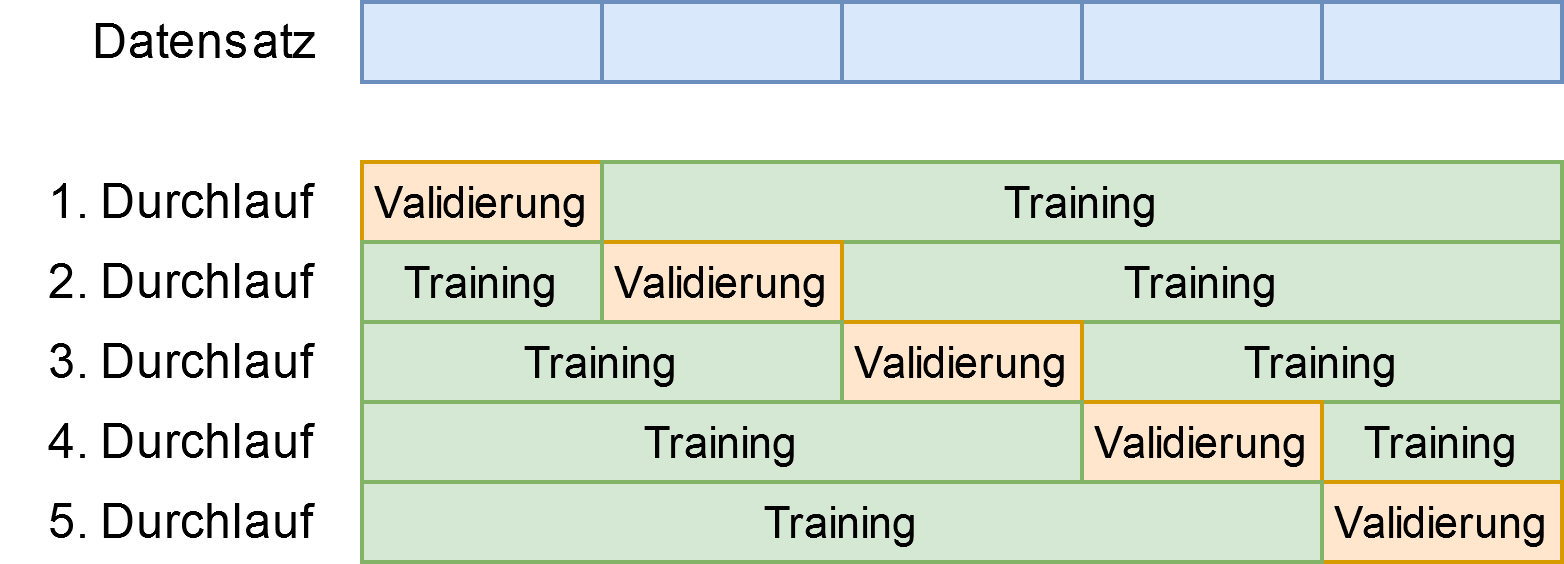
\includegraphics[width=0.90\textwidth]{kreuzvalidierung}
	\vspace*{-3mm}
	\caption[Beispiel für Kreuzvalidierung]{Beispiel für eine 5-fache Kreuzvalidierung \cite[S.44]{BA}.}
	\label{fig:crossvalidation}
\end{figure}
\vspace*{-5mm}
\subsection{Neuronale Netze}
In dieser Arbeit wurde sich wie heutzutage typisch bei der Bilderkennung auf Neuronale Netze und besonders die Konvolutionellen Neuronale Netze fokussiert. Diese sind bei der Bilderkennung in vielen Bereichen State of the Art und werden von vielen bekannten vortrainierten Modellen wie dem VGG19 genutzt. Um diese zu verstehen, sollen allerdings erst die einfachen Neuronalen Netze beschrieben werden.
\subsubsection{Biologische Grundlagen}
Neuronen sind für viele Menschen vor allem aus ihren eigenen Gehirn bekannt. In diesem arbeiten viele der kleinen Nervenzellen zusammen, um Informationen zu verarbeiten. Jedes Neuron nimmt elektrische Signale über seine stark verzweigten Dendriten auf und sammelt sie in seinem Zellkörper, dem Soma an. Ist eine gewissen stärke des elektrischen Signals vorhanden, so gibt ein Neuron dieses über sein Axon weiter. Axone sind lange, verzweigte Fäden, die mittels Synapsen mit den Dendriten anderer Neuronen verbunden sind. Synapsen arbeiten mit chemischen Transmittern und können eine erregende oder hemmende Wirkung auf das zu übertragene Signal haben. Biologische Neuronale Netze lernen nun, indem die Stärke der Verbindung über die Synapsen gesteuert wird. Außerdem können Verbindungen getrennt und neu eingegangen werden, was ebenfalls einen Lerneffekt erzeugt \cite[S.24]{BA}\cite[S.43-45]{DEEP_LEARNING}\cite[S.29-30]{NNP}.
\begin{figure}[H]
	\centering
	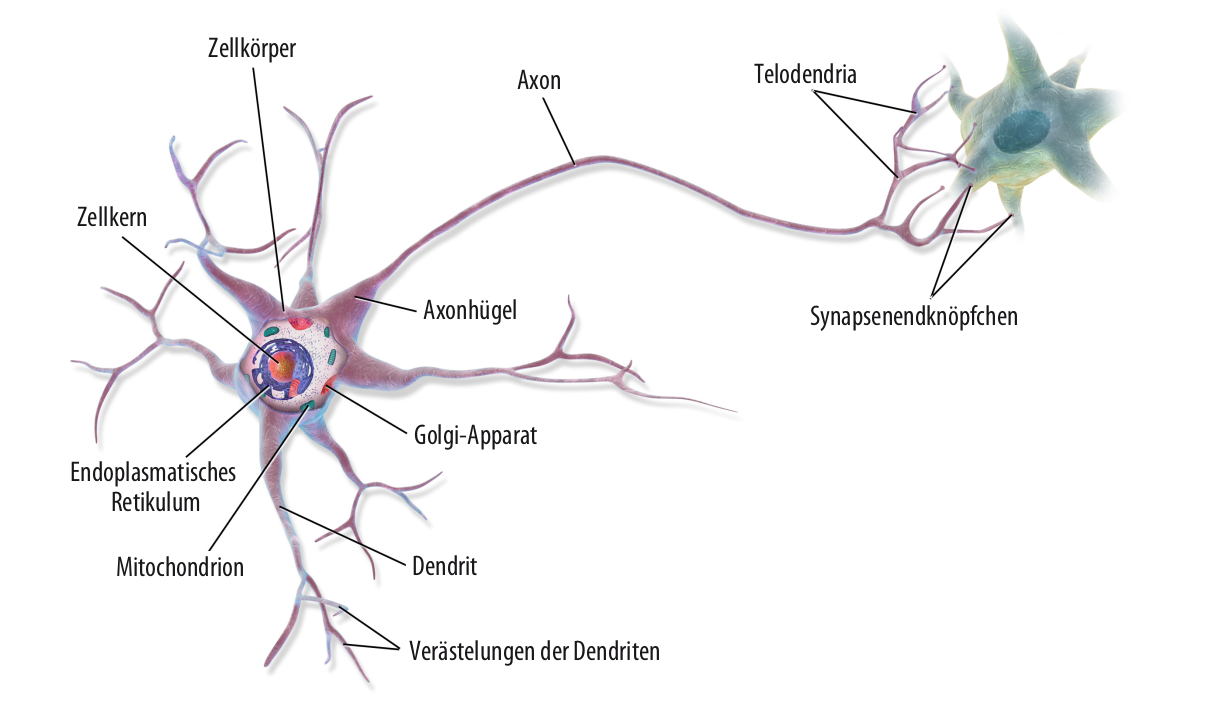
\includegraphics[width=1\textwidth]{neuron_biologisch}
	\vspace*{-5mm}
	\caption[Aufbau eines biologischen Neurons]{Aufbau eines biologischen Neurons \cite[S.255]{MACHINE_LEARNING}.}
	\label{fig:aufbau_bio_neuron}
\end{figure}
\vspace*{-5mm}
\subsubsection{Künstliche Neuronen}
In künstlichen Neuronalen Netzen wird nun eine auf den Biologischen Grundlagen basierende künstliche Variante von Neuronen genutzt. Diese nehmen über ihre Eingänge, ähnlich zu den verbundenen Axonen, Signale auf, welche im Folgenden als ein Vektor \textbf{x} mit n-Elementen dargestellt wird. Jede dieser Eingangssignale wird nun über einen eigenen Wert in einem Gewichtungsvektor \textbf{w} gehemmt oder verstärkt, was ähnlich zu der Arbeitsweise von Synapsen ist. Nun, werden ebenfalls ähnlich zum biologischen Vorbild, alle eingegangen Signale aufaddiert, jedoch an eine Aktivierungsfunktion \ensuremath{f_{akt}} weitergegeben, welche ein Signal nochmal auf eine bestimmte Weise verarbeitet und sich komplett anders zum biologischen Vorbild verhalten kann. Zum Schluss kann das errechnete Signal des Künstlichen Neurons an weitere Neuronen geleitet werden, ähnlich zum ausgehenden Axon der biologischen Variante \cite[S.25]{BA}\cite[S.30-31]{NNP}.
\begin{figure}[H]
	\centering
	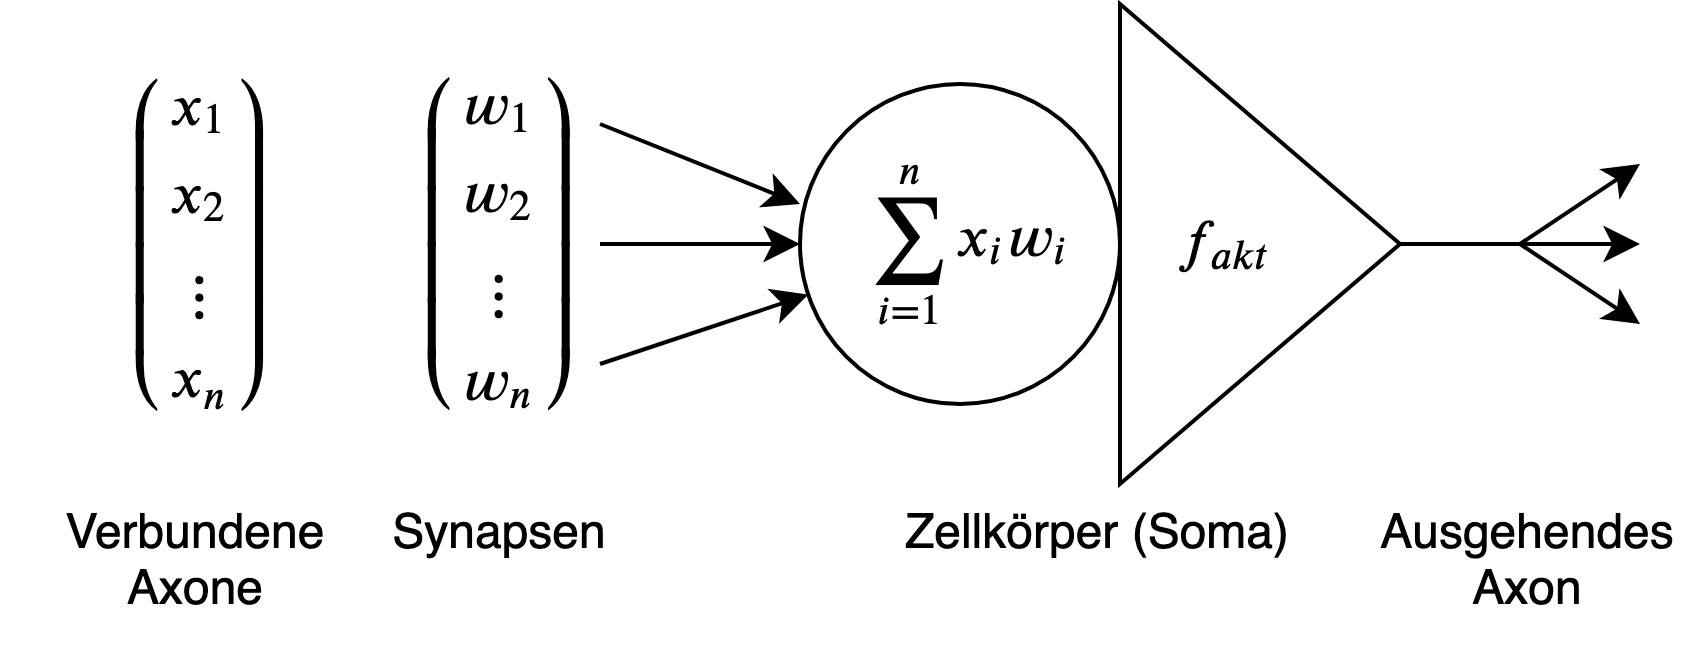
\includegraphics[width=1\textwidth]{neuron_adv}
	\vspace*{-5mm}
	\caption[Aufbau eines künstlichen Neurons]{Aufbau eines künstlichen Neurons, angelehnt an das biologische Vorbild \cite[S.25]{BA}.}
	\label{fig:aufbau_kuenstliches_neuron}
\end{figure}
\vspace*{-5mm}
Für n-Eingänge lässt sich ein Künstliches Neuron nun folgendermaßen definieren \cite[S.25]{BA}\cite[S.30]{NNP}:
\begin{equation}
\label{eq:perceptron_def}
\begin{aligned}
y = f_{akt}\left(\sum_{i=1}^{n}x_iw_i\right) = f_{akt}(\textbf{x}^T \cdot \textbf{w})
\end{aligned}
\end{equation}\myequations{Mathematische Definition eines Künstlichen Neurons}\\
Wird eine Schwellenwertfunktion \eqref{eq:heavyside} als Aktivierungsfunktion genutzt, so wird ein Künstliches Neuron in der Regel als Perzeptron bezeichnet \cite[S.26]{BA}\cite[S.49]{DEEP_LEARNING}. 
\begin{equation}
\label{eq:heavyside}
\begin{aligned}
f_{akt} =
\begin{cases}
0 & x < 0\\
1 & x \geq 0
\end{cases}
\end{aligned}
\end{equation}\myequations{Schwellenwertfunktion eines Perzeptrons}
\subsubsection{Einschichtige Neuronale Netze}
Liegen mehrere Künstliche Neuronen oder Perzeptrons in einer einzigen Schicht vor, entsteht ein erstes einschichtiges Neuronales Netz. Dabei wird jeder Eingang in das Neuronale Netz mit jedem Neuron in der einen Schicht des Netz verbunden und über Gewichtungen verändert. Die Eingänge werden dabei häufig in der Notation als Schicht von Eingabeneuronen dargestellt, welche lediglich die Eingabewerte an die Künstlichen Neuronen weitertragen. Weiterhin wird in die Eingabeschicht dieser Netze häufig ein spezielles Neuron eingeführt, welches lediglich eine Eins als Ausgabe liefert und über Gewichtungen verändert werden kann. Dies wird als Bias-Neuron bezeichnet. Die Ausgänge der Künstlichen Neuronen des Netzes, können nun als Ausgabevektor \textbf{y} ausgelesen werden \cite[S.26]{BA}\cite[S.258]{MACHINE_LEARNING}. Ein einschichtiges Neuronale Netz mit einer vereinfachten Darstellung der Neuronen ist in der Abbildung \ref{fig:multi_neuron_perceptron} dargestellt.
\begin{figure}[H]
	\centering
	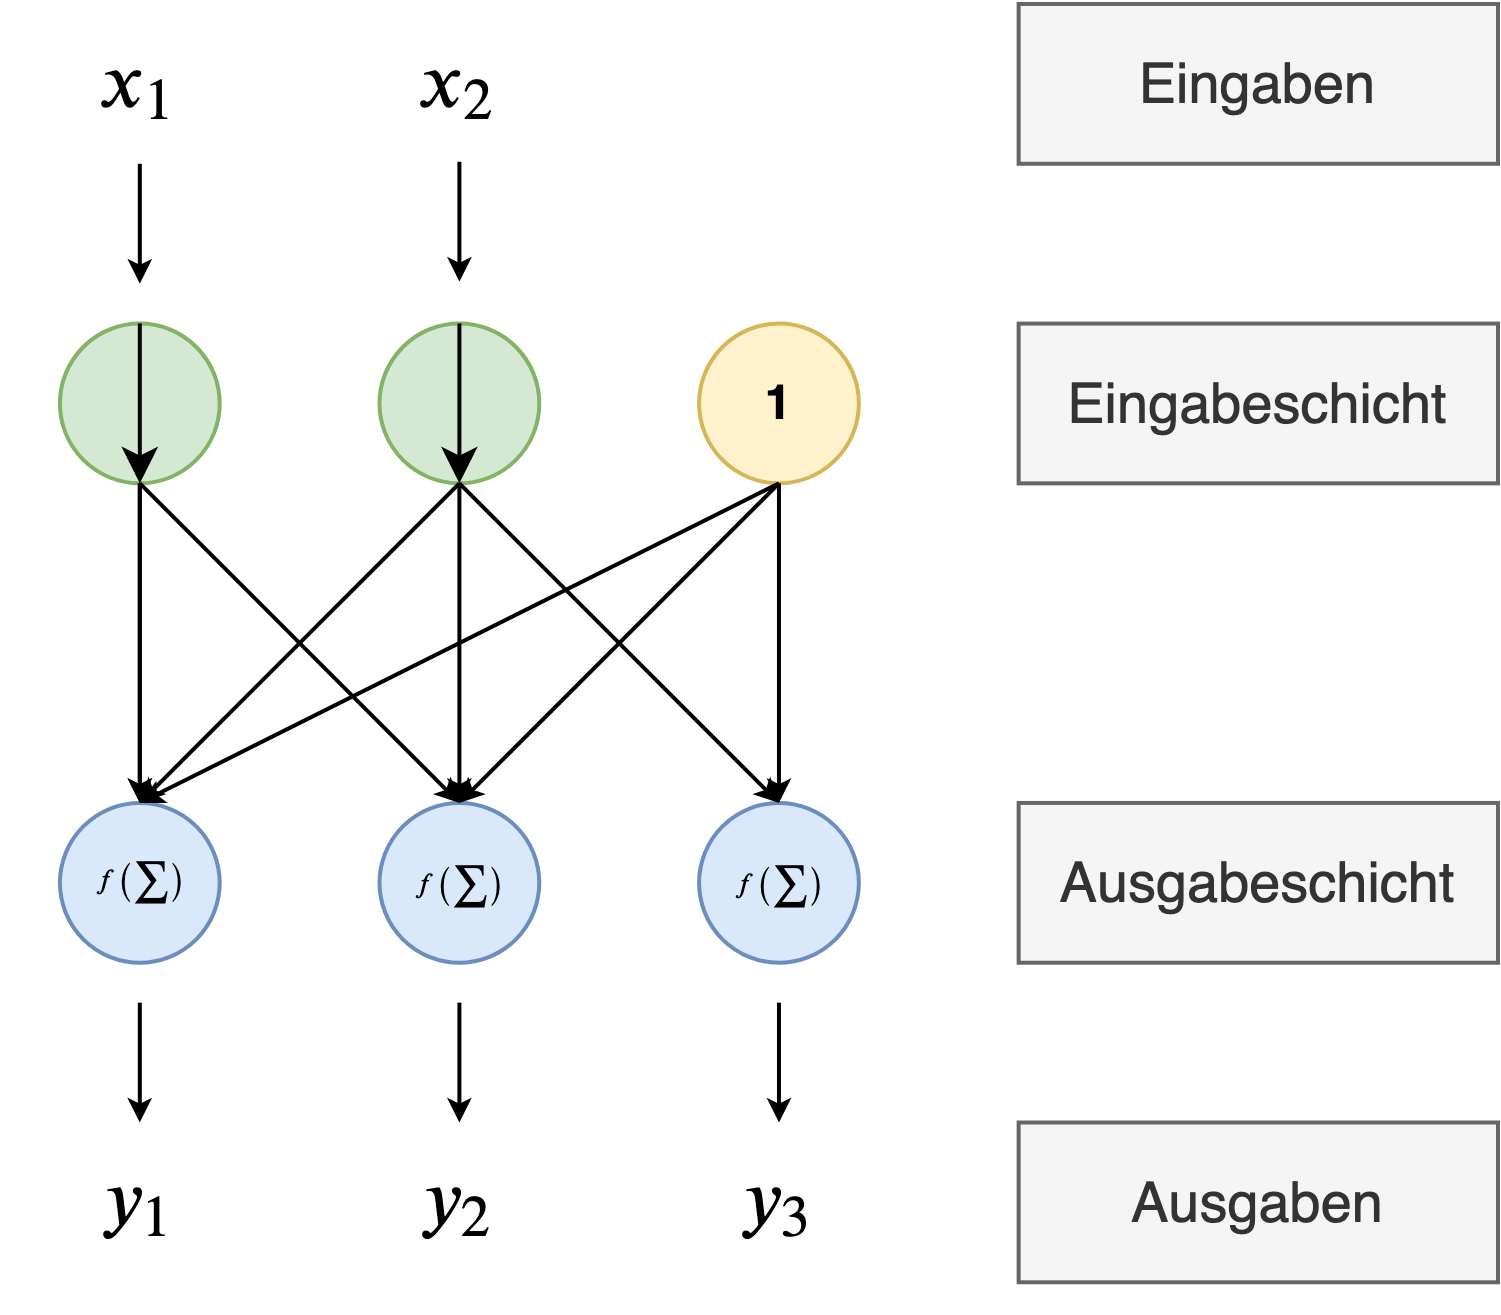
\includegraphics[width=0.7\textwidth]{multi_neuron_perceptron}
	\vspace*{-5mm}
	\caption[Einschichtiges Neuronales Netz]{Aufbau eines einschichtigen Neuronalen Netzes \cite[S.27]{BA}\cite[S.258]{MACHINE_LEARNING}.}
	\label{fig:multi_neuron_perceptron}
\end{figure}
\vspace*{-5mm}
Die Gewichtungen zwischen der Eingabeschicht und der Ausgabeschicht werden zur einfachen Berechnung typischerweise als Matrix \textbf{W} dargestellt \eqref{eq:perzeptron_matrix} \cite[S.26]{BA}\cite[S.258]{MACHINE_LEARNING}.
\begin{equation}
\label{eq:perzeptron_matrix}
\begin{aligned}
\textbf{W} = 
\begin{pmatrix}
w_{11} & w_{12} & w_{13} \\
w_{21} & w_{22} & w_{23} \\
w_{b1} & w_{b2} & w_{b3} \\\end{pmatrix}
\end{aligned}
\end{equation}\myequations{Matrizendarstellung eines einschichtigen Neuronalen Netzes}\\ 
Mittels dieser Darstellung kann bei einer elementweisen Auswertung der Aktivierungsfunktion und einer Matrizenmultiplikation sehr einfach eine ähnliche Formel wie \eqref{eq:perceptron_def} angewandt werden, um die Ausgabe des Netzes zu errechnen:
\begin{equation}
\label{eq:slp_def}
\begin{aligned}
\textbf{y} = f_{akt}(\textbf{x}^T \cdot \textbf{W})
\end{aligned}
\end{equation}\myequations{Mathematische Definition eines einschichtigen Neuronalen Netzes}\\
Doch wie lernen einschichtige Neuronale Netze sich an neue Informationen anzupassen. Früher und für nicht überwachtes Lernen, wurde hier häufig die an die menschliche Biologie angelehnte Hebbsche Lernregel angewandt. Diese ist jedoch für überwachtes Lernen wie im Fall der Problemstellung eher ungeeignet. Es wird also das in der Praxis häufig eingesetzte Gradientenabstiegsverfahren betrachtet \cite[S.259]{MACHINE_LEARNING}. 
\subsubsection{Gradientenabstiegsverfahren} 
Die Idee hinter dem Gradientenabstiegsverfahren ist eine schrittweise Verringerung des Gesamtfehler eines einschichtigen Neuronalen Netzes \ensuremath{F} unter einer Fehlerfunktion \ensuremath{E(\textbf{y'}, \textbf{y})} für die Vorhersagen \ensuremath{\textbf{y'}} und die Labels \ensuremath{\textbf{y}}, indem eine optimale Kombination von Gewichten \ensuremath{\textbf{W}_{min}} gesucht wird \eqref{eq:gradient} \cite[S.28]{BA}.
\begin{equation}
\label{eq:gradient}
\begin{aligned}
\underset{\textbf{W}}{\text{min}} \medspace & & & F = E(f_{akt}(\textbf{x}^T \cdot \textbf{W}) ,y)
\end{aligned}
\end{equation}\myequations{Ziel des Gradientenabstiegsverfahren}\\
In einer dreidimensionalen Gebirgslandschaft, welche durch zwei Gewichte und dem Fehler beschrieben ist, kann man sich die Arbeitsweise dieses Algorithmus leicht vorstellen. Ein Bergsteiger mit eingeschränkter Sicht in dieser Landschaft, kann sich lediglich über den Punkt des steilsten Abstiegs langsam und schrittweise in ein Tal wagen. Er versucht also immer weiter dem steilsten Abstieg zu folgen, bis er ein Tal der Fehlerfunktion findet. Dies lässt sich in \ref{fig:gradient} erkennen \cite[S.28]{BA}\cite[S.39]{NN}. 
\begin{figure}[H]
	\centering
	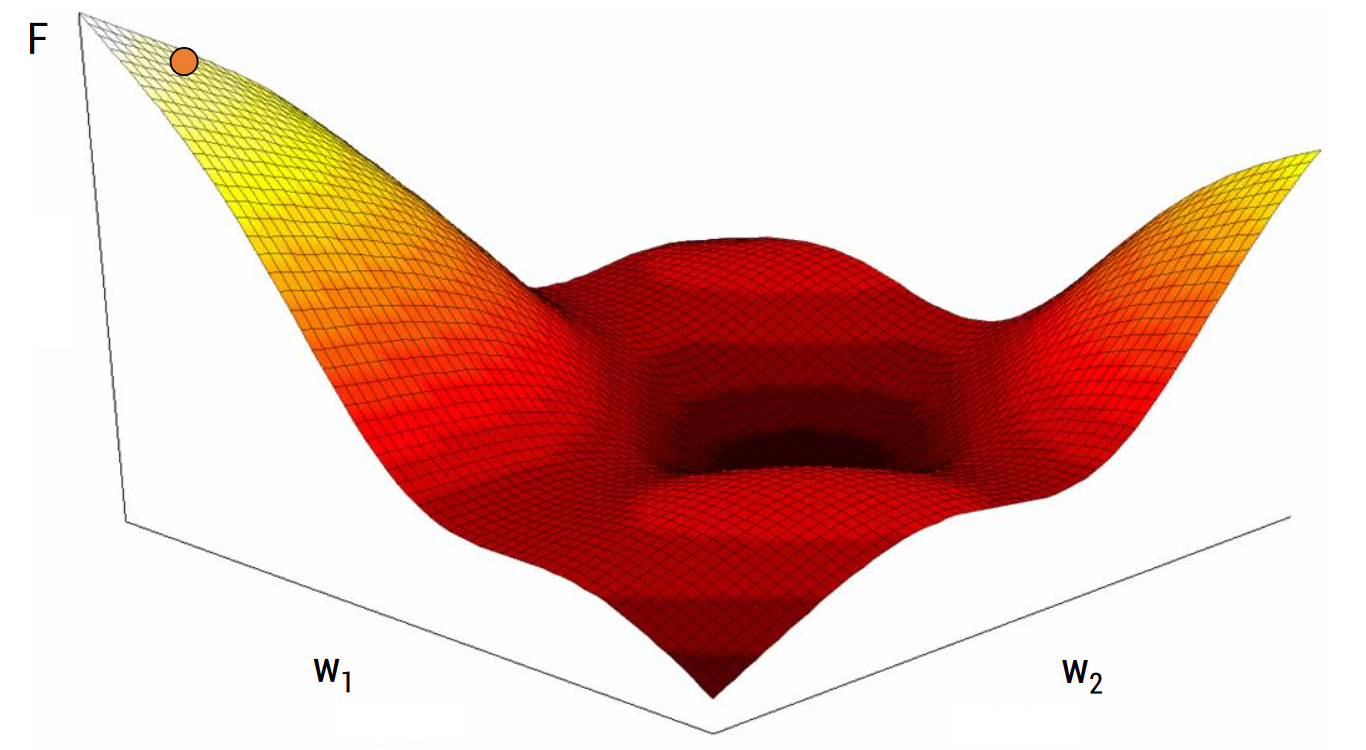
\includegraphics[width=1.0\textwidth]{gradient}
	\vspace*{-5mm}
	\caption[Fehler im Neuronalen Netz]{Gebirgslandschaft des Fehlers in einem Neuronalen Netz \cite{GRADIENT_IMAGE}.}
	\label{fig:gradient}
\end{figure}
Im Algorithmus funktioniert dies durch partielle Ableitungen der Fehlerfunktion nach jedem Gewicht und einem Anwenden des daraus resultierenden Gradientenvektors in negativer Richtung angepasst durch die gewählte Lernrate, welche die Geschwindigkeit des Abstiegs zum Minimum definiert. Dies wird wiederholt bis ein gewünschtes Minimum oder eine gewählte Zahl an Wiederholungen erreicht wurde. Die Wiederholungen werden bei Neuronalen Netzen über alle Trainingsdaten auch als Epochen bezeichnet \cite[S.29-30]{BA}\cite[S.41]{NN}\cite[S.31]{DEEP_LEARNING}. Häufig wird jede Epoche aber auch noch in kleinere Teile, den sogenannten Batches unterteilt.
\begin{figure}[H]
	\centering
	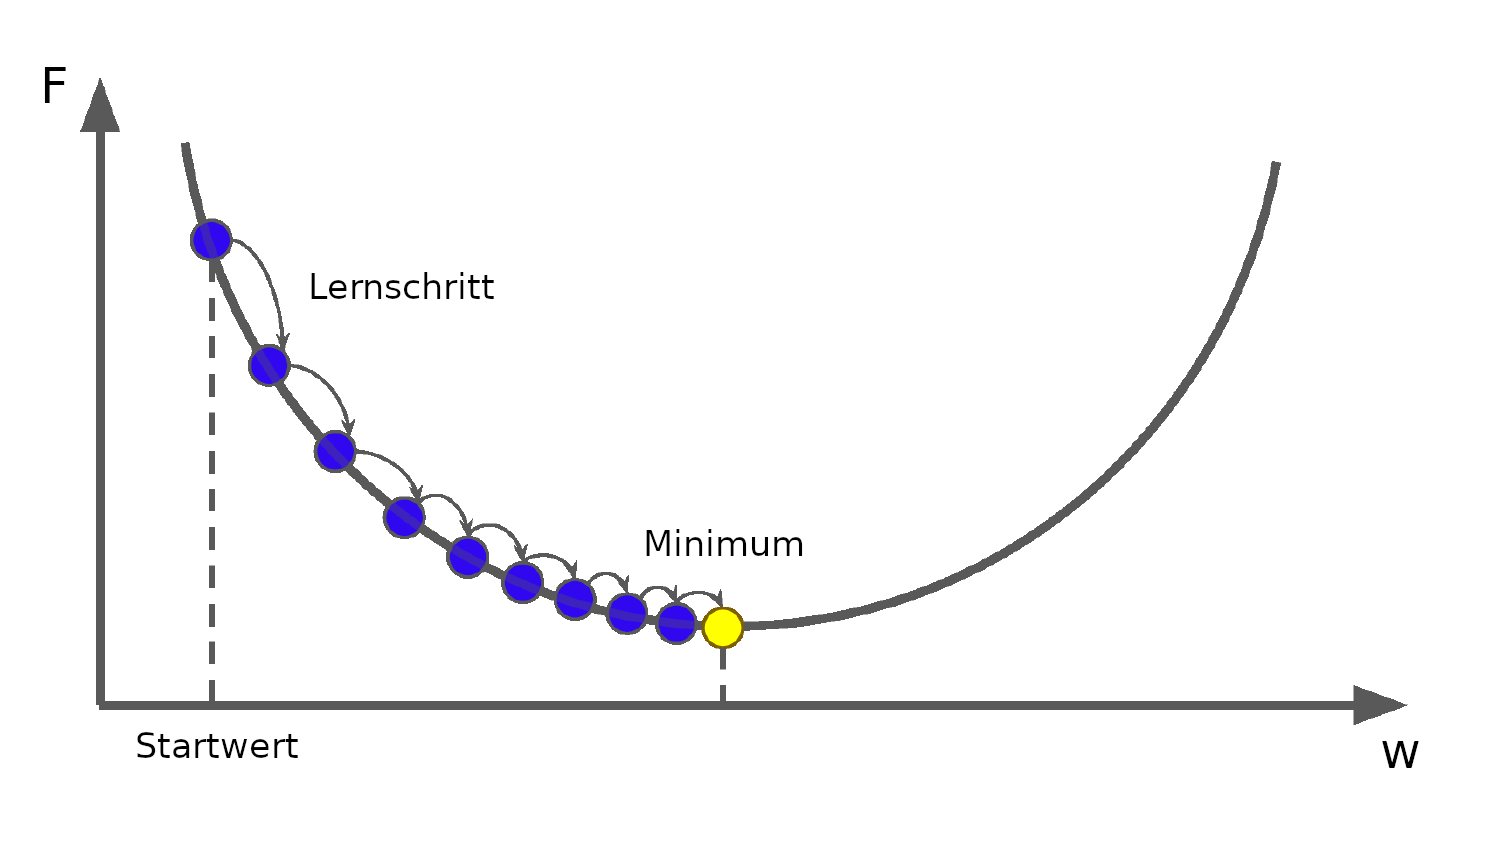
\includegraphics[width=0.8\textwidth]{2DGradient}
	\vspace*{-5mm}
	\caption[Gradientenabstiegsverfahren in zwei Dimensionen]{Das Gradientenabstiegsverfahren in zwei Dimensionen \cite[S.113]{MACHINE_LEARNING}.}
	\label{fig:2DGrad}
\end{figure}
\vspace*{-5mm}
Bereits durch die Beschreibung des Algorithmus lassen sich einige Probleme abschätzen. Zum einen ist nicht gewährleistet, dass ein globales Minimum gefunden wird. Stoppt der Algorithmus in einem lokalen Minimum, so kann nicht weiter optimiert werden. Eine höhere Lernrate oder ein Momentum-Term, welcher dem Algorithmus beim Wander durch die mehrdimensionale Gebirgslandschaft eine gewisse Trägheit gibt, können dafür sorgen, dass lokale Minima übersprungen werden. Eine hohe Lernrate kann aber auch zu Problemen führen. So ist in diesem Fall eine ein- oder mehrschrittige Oszillation zwischen den Talrändern ein typisches Problem, welches auftreten kann. Auch kann sie ganz zum Überspringen des globalen Minimum führen \cite[S.30]{BA}\cite[S.46-47]{NN}.
\\\\
Ein weiteres Problem tritt bezüglich der bisher bekannten Aktivierungsfunktion, der Schwellenwertfunktion, auf. Für diese kann kein Gradient ungleich null berechnet werden, wodurch kein Minimum gefunden werden kann. Dies kann durch das Einführen anderer Aktivierungsfunktionen gelöst werden und wird in einem späteren Kapitel betrachtet \cite[S.31-32]{BA}\cite[S.262]{MACHINE_LEARNING}.
\subsubsection{Mehrschichtige Neuronale Netze}
Leider lassen sich mit einschichtigen Neuronalen Netzen nur einfache Probleme lösen. Dies lässt sich durch das Einfügen weiterer Schichten lösen, indem die Ausgaben der vorherigen Schicht durch weitere erlernbare Gewichtungen an die nächste Schicht weitergegeben werden. Alle Schichten zwischen der Eingabe- und Ausgabeschicht werden dabei als verborgene Schichten oder Hidden-Layer bezeichnet \cite[S.31-32]{BA}\cite[S.261]{MACHINE_LEARNING}. Ein Beispiel hierfür ist in der folgenden Abbildung zu erkennen: 
\begin{figure}[H]
	\centering
	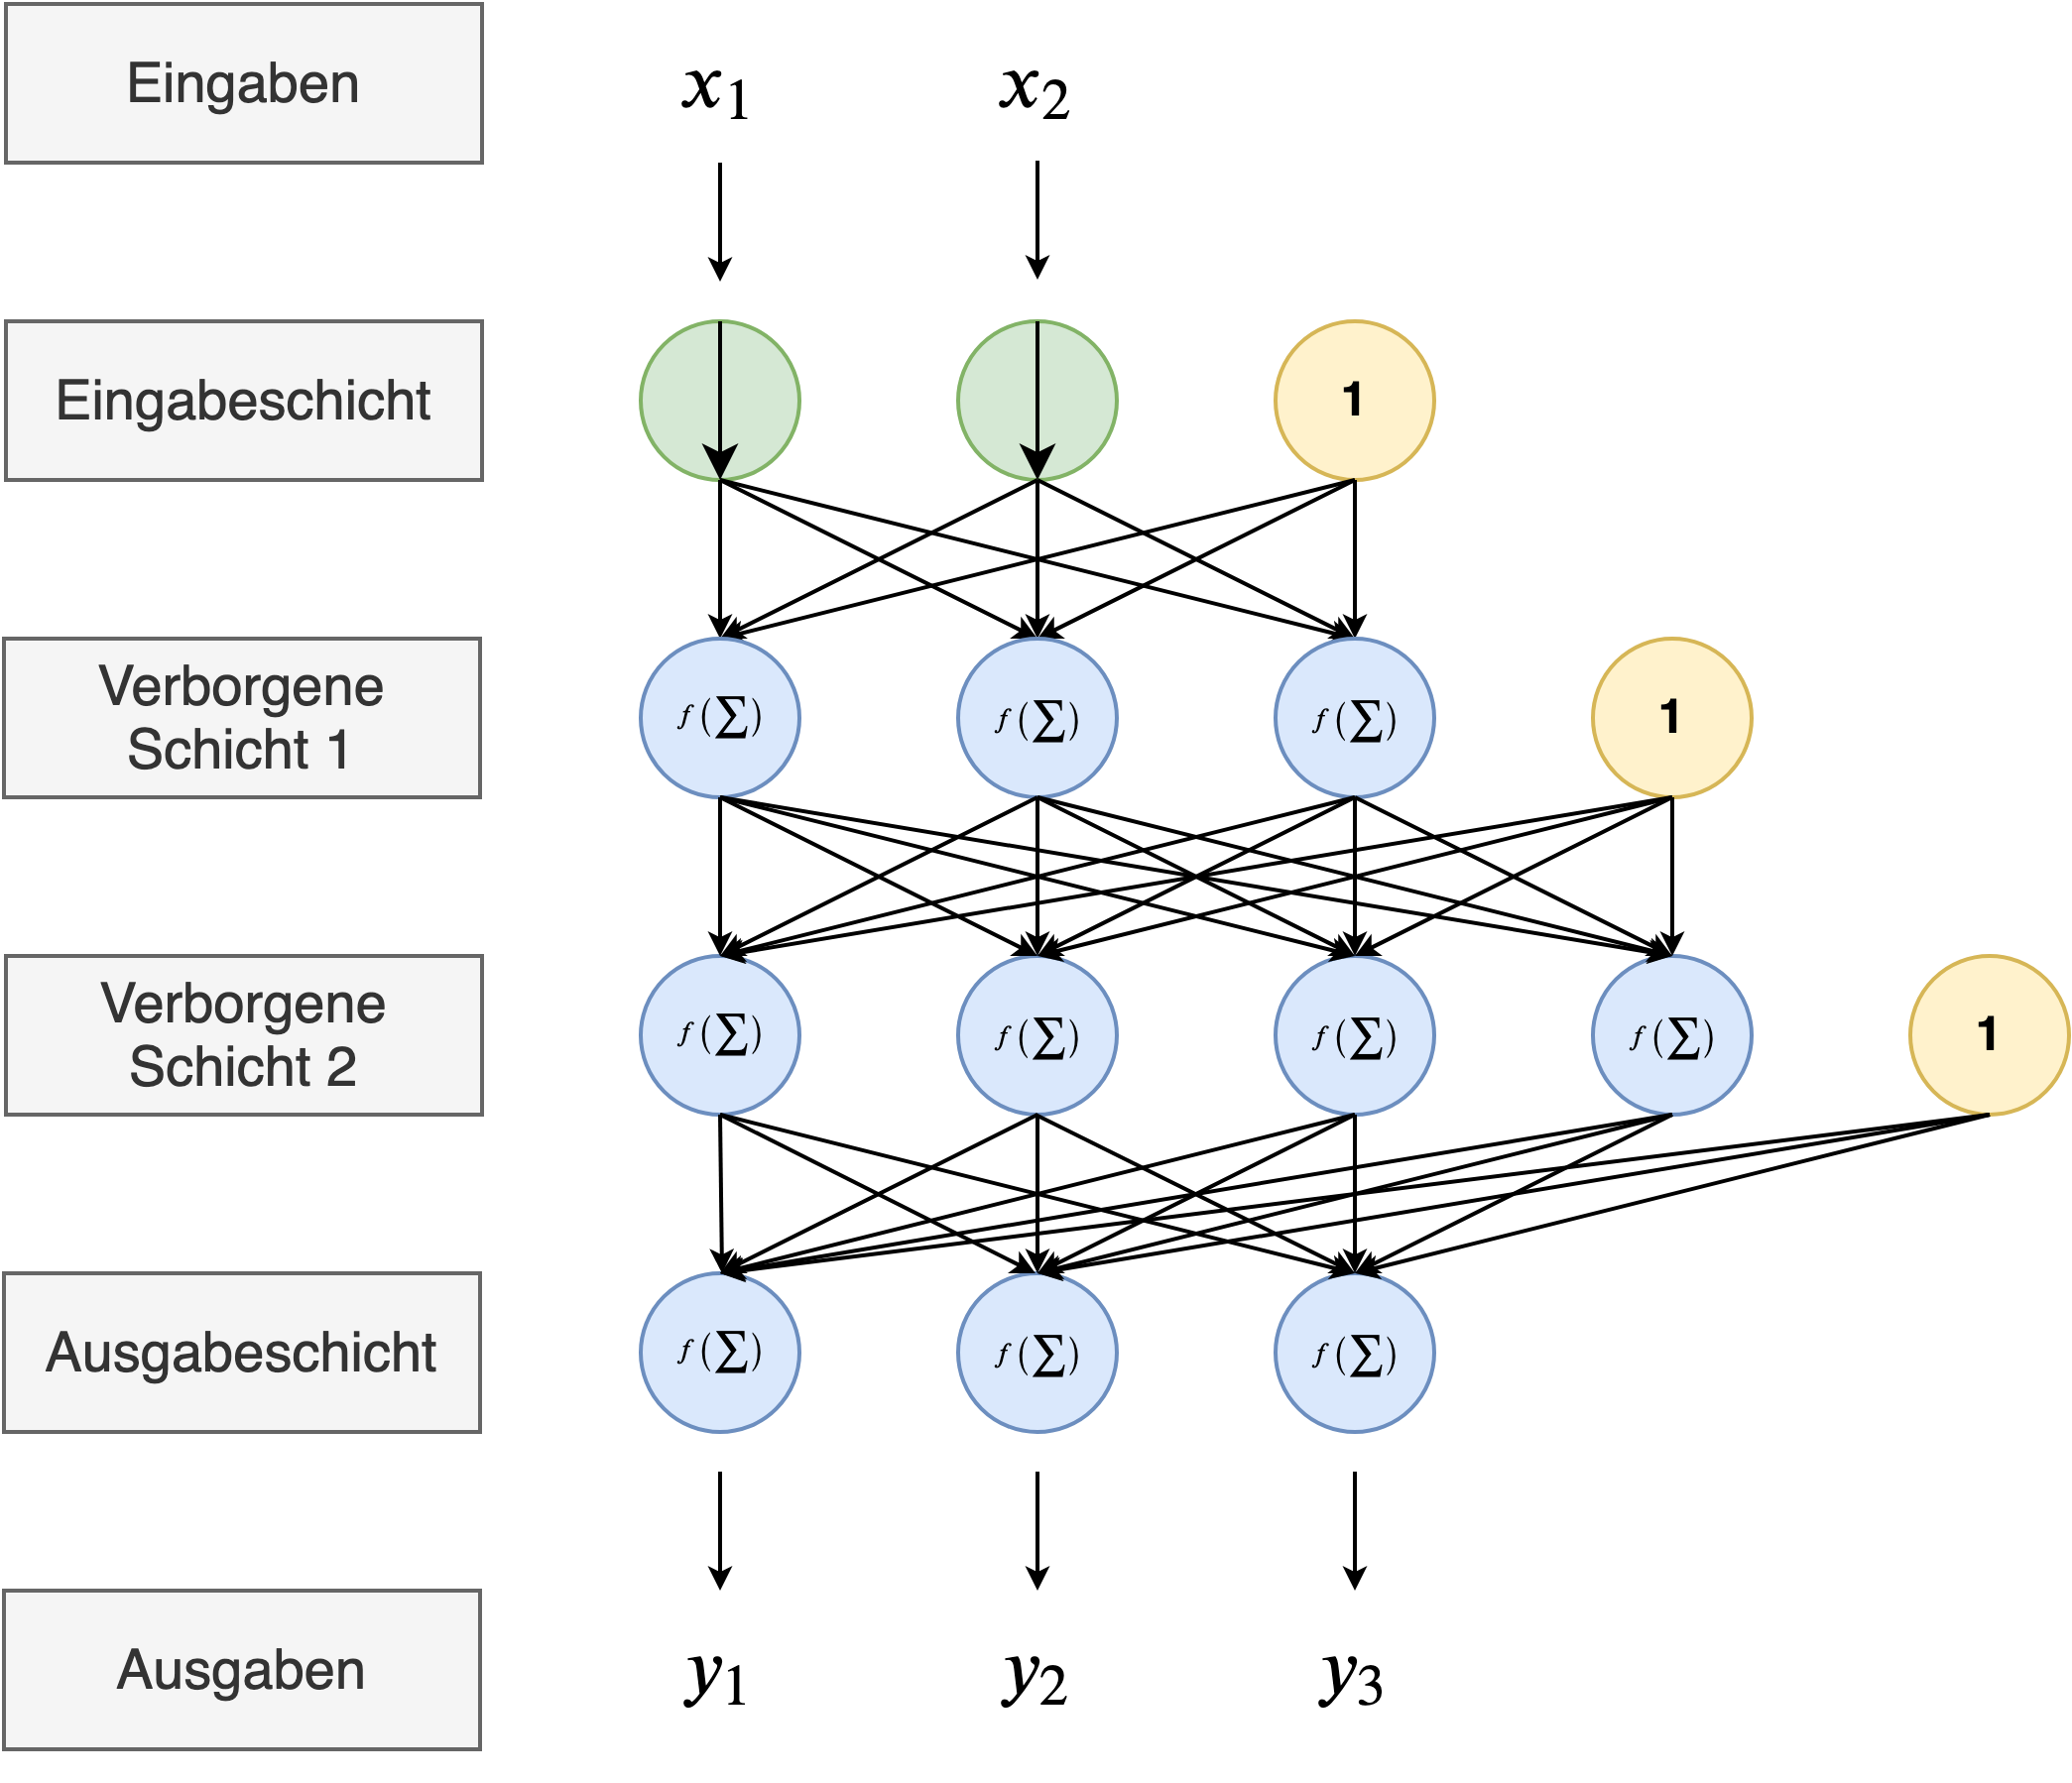
\includegraphics[width=0.85\textwidth]{multi_layer_perceptron}
	\vspace*{-3mm}
	\caption[Mehrschichtiges Neuronales Netz]{Ein mehrschichtiges Neuronales Netz mit zwei verborgenen Schichten \cite[S.32]{BA}\cite[S.261]{MACHINE_LEARNING}.}
	\label{fig:mutlilayer_nn}
\end{figure}
\vspace*{-5mm}
Leider funktioniert das Gradientenabstiegsverfahren in der bisherigen Funktionsweise nur mit einem einzigen Layer, da der Fehler von verborgenen Schichten nicht direkt errechnet werden kann. Es fehlt damit eine Lernmethode für das überwachte Lernen. Die Lösung hierfür ist das Backpropagation-Verfahren \cite[S.261]{MACHINE_LEARNING}. 
\subsubsection{Backpropagation-Verfahren}
Über das Backpropagation-Verfahren wird der Fehler eines mehrschichtigen Neuronalen Netzes über seine Schichten zurückgerechnet, um eine Veränderungen der Gewichtungen in den verborgenen Schichten zu ermöglichen \cite[S.51-52]{NN}.
\\\\
Das Backpropagation-Verfahren wird folgendermaßen ausgeführt. Nachdem die Netzausgabe bestimmt wurde, wird für diese der Fehler zu den gewünschten Ausgaben errechnet. In der Ausgabeschicht wird mit dem Gradientenabstiegsverfahren für jedes Gewicht der negative Gradient zum letzten Hidden-Layer errechnet. Dieser wird nun durch die Gewichte der verbundenen Hidden-Neuronen zurückgerechnet und damit auf diese verbundenen Hidden-Neuronen verteilt. Wird dies für alle Neuronen der betrachteten Schicht wiederholt, kann mittels des Gradientenabstiegsverfahren der Fehler der verbundenen verborgenen Schicht errechnet werden. Dies wird wiederholt, bis die Eingabeschicht erreicht wurden \cite[S.33]{BA}\cite[S.52-53]{NN}. Wurden die Gradienten errechnet, können die Gewichtungen mit einem vorher definierten Lernparameter angepasst werden \cite[S.262]{MACHINE_LEARNING}. Der Algorithmus wird nun batch- und epochenweise solange wiederholt, bis der Fehler ein Limit unterschreitet oder eine maximale Anzahl an Wiederholungen erreicht wurde \cite[S.52]{NN}.
\\\\
Typischerweise können bei dem Backpropagation-Verfahren ähnliche Probleme wie beim Gradientenabstiegsverfahren auftreten. Außerdem können Gradienten aufgrund des Zurückrechnens sehr klein ausfallen und zu einer immer kleiner werdenden Anpassung der Gewichte in den ersten Schichten führen. Dies würde zu einem immer kleiner werdenden Lerneffekt führen. In wenigen Fällen kann auch ein gegenteiliges Problem, die explodierenden Gradienten auftreten \cite[S.33-34]{BA}\cite[S.275-276]{MACHINE_LEARNING}. In der Regel lässt sich dies über sinnvollere Aktivierungsfunktionen und spezielle Regularisierungsverfahren lösen, die in den nächsten Kapiteln betrachtet werden. 
\subsubsection{Aktivierungsfunktionen}
Moderne Neuronale Netze verwenden in der Regel Aktivierungsfunktionen, welche auf der ReLU (Rectified Linear Units) basieren. Die ReLU hat im Gegensatz zu anderen, typischerweise früher eingesetzten Aktivierungsfunktionen wie der Sigmoidfunktion oder dem Tangens hyperbolicus, den Vorteil, dass sie keinen Sättigungseffekt, daher eine sehr kleine Ableitung, für positive Werte erfährt. Dies wirkt dem Problem der schwindenden Gradienten entgegen \cite[S.34-35]{BA}. Für die Eingabe x ist die ReLU definiert als \cite[S.245, S.279]{MACHINE_LEARNING}:
\begin{equation}
\label{eq:relu}
\begin{aligned}
f_{akt} =
\begin{cases}
x & x \geq 0\\
0 & x < 0
\end{cases}
\end{aligned}
\end{equation}\myequations{ReLU}\\
Wie zu sehen ist die ReLU für positive Werte lediglich äquivalent zu der originalen Eingabe. Damit ist sie sehr einfach zu berechnen. Leider leidet sie unter einem großen Problem. Ein Neuron mit einer negative Eingabesumme vor der Aktivierungsfunktionen liefert eine Konstante 0 und trägt mich mehr zum Lernen bei. Tritt dies bei vielen Neuronen auf, kann dies ebenfalls den Lerneffekt beschränken \cite[S.279]{MACHINE_LEARNING}.
\\\\
In vielen Fällen wird dies über die Verwendung leicht abgewandelter ReLU-Varianten wie der Leaky-ReLU oder der ELU (Exponential Linear Unit), die auch in diesem Projekt verwendet wurde, gelöst. Die ELU hat im Positiven ein lineares Verhalten, während sie sich im Negativen wie eine negative Exponentialfunktion verhält die sich einem Parameter a annähert. Es gilt \cite[S.36]{BA}:
\begin{equation}
\label{eq:elu}
\begin{aligned}
f_{akt} =
\begin{cases}
x & x \geq 0\\
a(e^x - 1) & x < 0
\end{cases}
\end{aligned}
\end{equation}\myequations{ELU}\\
Mit diesen Aktivierungsfunktionen können bereits einige typische Probleme beim Maschinellen Lernen mit mehrschichtigen Neuronalen Netzen und Backpropagation verhindert werden. Eine weitere verwendete Aktivierungsfunktion, welche vorallem bei der Ausgabeschicht von Klassifikationsproblemen mit One-Hot kodierten Labeln nützlich ist, ist die Softmax-Funktion. Im Gegensatz zu anderen Aktivierungsfunktionen erhält sie die Ausgabe aller Neuronen einer Schicht. Diese Ausgaben werden dann mit der Summe aller Ausgaben normalisiert, was in einen Vektor von Zahlen zwischen 0 und 1 resultiert. Diese werden in der Regel als Wahrscheinlichkeiten für eine vorliegende Klasse interpretiert. Für den Vektor mit Neuronensummen \ensuremath{\textbf{s}} mit n-Elementen ist die Softmax definiert als \cite[S.37]{BA}\cite[S.141-142, S.263]{MACHINE_LEARNING}: 
\begin{equation}
\label{eq:softmax}
\begin{aligned}
f_{akt} = \frac{e^{s_i}}{\sum_{i=1}^{n}e^{s_i}}
\end{aligned}
\end{equation}\myequations{Softmax}
\subsubsection{Regularisierungsverfahren}
Zuletzt werden nun zwei typische Regularisierungsverfahren für Neuronale Netze betrachtet, mit denen die Performanz dieser auf bestimmte Weisen erhöht werden kann.
\\\\
Die Batch-Normalisierung ist ein ideales Verfahren, um schwindenden Gradienten sowie Overfitting entgegen zu wirken und die Stabilität von Neuronalen Netzen zu erhöhen. Diese wird schicht- und batchweise ausgeführt, indem die Summe aller Neuronen einer Schicht vor der Aktivierungsfunktion standardisiert wird. Das Verfahren arbeitet, indem der Mittelwert auf 0 zentriert und durch die Standardabweichung der Batch geteilt wird. Dann wird das Ergebnis über zwei lernbare Parameter skaliert und verschoben. Dadurch kann das Netz die ideale Skalierung und den Mittelwert der Eingaben für eine Schicht erlernen. Schwindenden Gradienten werden dadurch so stark bekämpft, dass sogar der Einsatz der Sigmoidfunktion oder des Tangens hyperbolicus wieder denkbar wäre \cite[S.37-38]{BA}\cite[S.282-283]{MACHINE_LEARNING}.
\\\\
Eine weitere Möglichkeit zur Regularisierung ist ein Dropout in verborgenen Schichten. Das Prinzip vom Dropout ist, dass Neuronen in einer Schicht während eines Schritts des Trainingsvorgangs mit einer gewissen Wahrscheinlichkeit ausgelassen werden. Wird der nächste Schritt erreicht, so werden die Dropouts neu ausgewürfelt. Durch das Auslassen von gewissen Neuronen, werden andere dazu gezwungen ihr Wissen zu verallgemeinern, da sie sich nicht auf die ausgeschiedenen Neuronen verlassen können. Dies wirkt Overfitting entgegen \cite[S.38-39]{BA}\cite[S.205-206]{NNP}.
\subsection{Konvolutionelle Neuronale Netze}
Heutzutage werden für Aufgaben der Bilderkennung in der Regel keine einfachen Neuronalen Netze, sondern Konvolutionelle Neuronale Netze eingesetzt. Diese wurden zum ersten mal 1980 eingesetzt und sind am Aufbau des visuellen Cortex des Menschen angelehnt. In diesem Arbeiten Neuronen in verschiedenen Schichten von Filtern, die aufeinander aufbauen. Die oberen Filter erkennen viele einfache Bildelemente, wie unterschiedliche Ausrichtungen von Linien. Diese werden weiter an untere Schichten geleitet, die das gefilterte immer weiter zu komplexen Mustern und Bildern kombinieren können \cite[S.360]{MACHINE_LEARNING}. 
\begin{figure}[H]
	\centering
	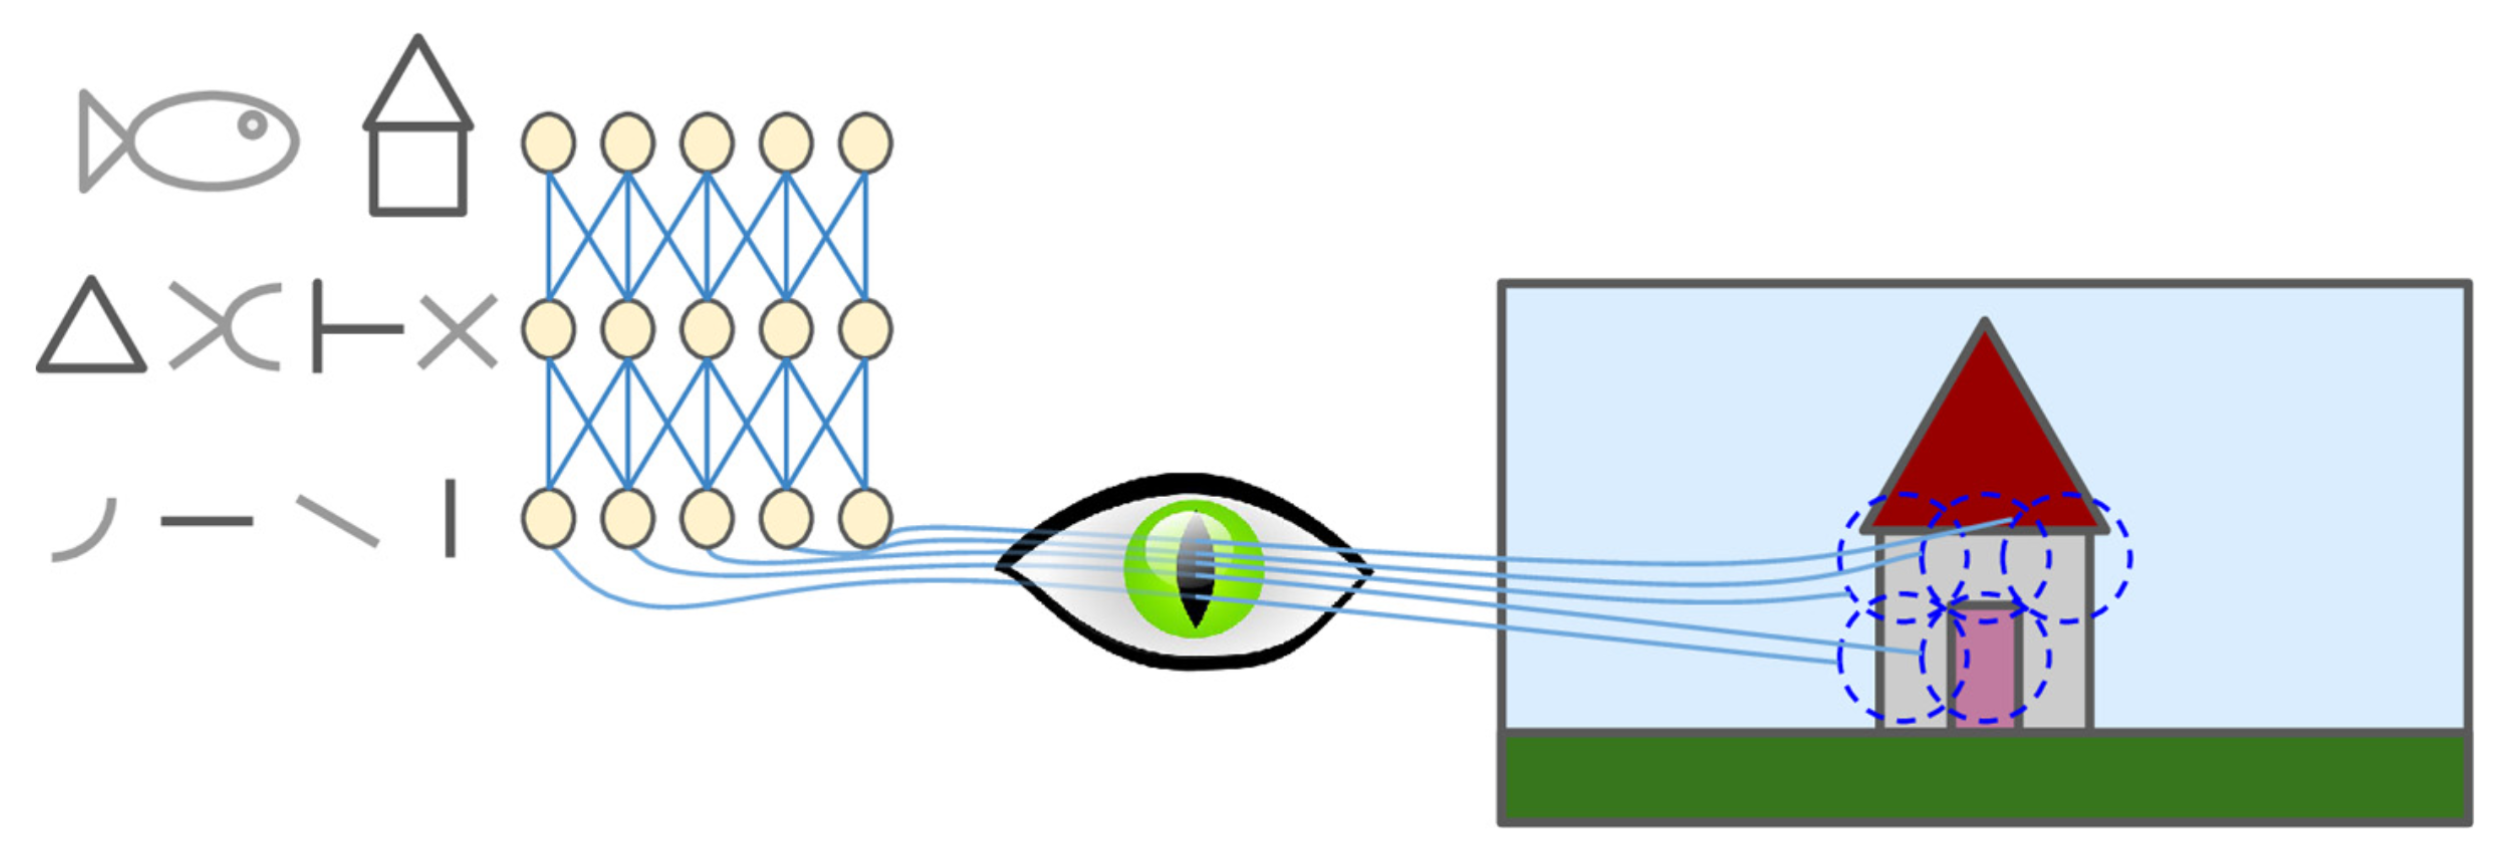
\includegraphics[width=0.85\textwidth]{visueller_cortex}
	\vspace*{-3mm}
	\caption[Aufbau des visuellen Cortex]{Aufbau des visuellen Cortex eines Menschen \cite[S.360]{MACHINE_LEARNING}.}
	\label{fig:visueller_cortex}
\end{figure}
\vspace*{-5mm}
Diese Erkenntnisse wurden dann genutzt, um 1980 die ersten Konvolutionelle Neuronale Netze zu entwickeln und für die Erkennung von handgeschriebenen Ziffern zu nutzen. Ein typischer Aufbau für Konvolutionelle Neuronale Netze besteht aus drei verschiedenen Schichten. Die letzten Schichten sind dabei in der Regel die bereits betrachteten vollständig verbundenen Neuronale Netz Schichten. Am Anfang befinden sich allerdings im Wechsel Convolutional und Pooling Layer, welche im folgenden betrachtet werden \cite[S.361]{MACHINE_LEARNING}.
\subsubsection{Convolutional Layer}
Convolutional Layer bestehen vom Grundprinzip aus einer zweidimensionalen Gewichtsmatrix von Neuronen einer gewissen Höhe und Breite, auch Filter genannt, welche mit einer bestimmten Schrittweite (Stride) über ein Eingabebild- oder ein bereits vorher durch einen Convolutional Layer betrachtetes Bild wandern. Der Filter multipliziert dabei in jedem durch die Schrittweite betrachtete Ausschnitt des Bildes, die Bildpunkte mit eigenen im Filter vorhandenen und lernbaren Gewichtungen. Dann werden die gewichteten Bildpunkte aufsummiert. Es entsteht ein neuer Bildpunkt, welcher wenn ein zum Filter passendes Feature betrachtet wurde, einen hohen Wert aufweisen wird. Damit Randpixel betrachtet werden können, muss abhängig von der Filtergröße ein Padding am Rand des Bildes hinzugefügt werden. Hier sind unterschiedliche Arten wie ein Zero-Padding, also ein Auffüllen des Rands mit Nullen, denkbar. In der Abbildung \ref{fig:cnn_filter} ist ein Convolutional Layer mit einer Filtergröße von 3x3 Pixeln, einer Schrittweite von 2 und ein Zero-Padding erkennbar. Bei dieser Schrittweise ist klar zu erkennen, dass das Bild durch diese verkleinert wird. Dies ist nützlich, da hierdurch Bildauflösungen verringert werden können \cite[S.361-363]{MACHINE_LEARNING}.
\begin{figure}[H]
	\centering
	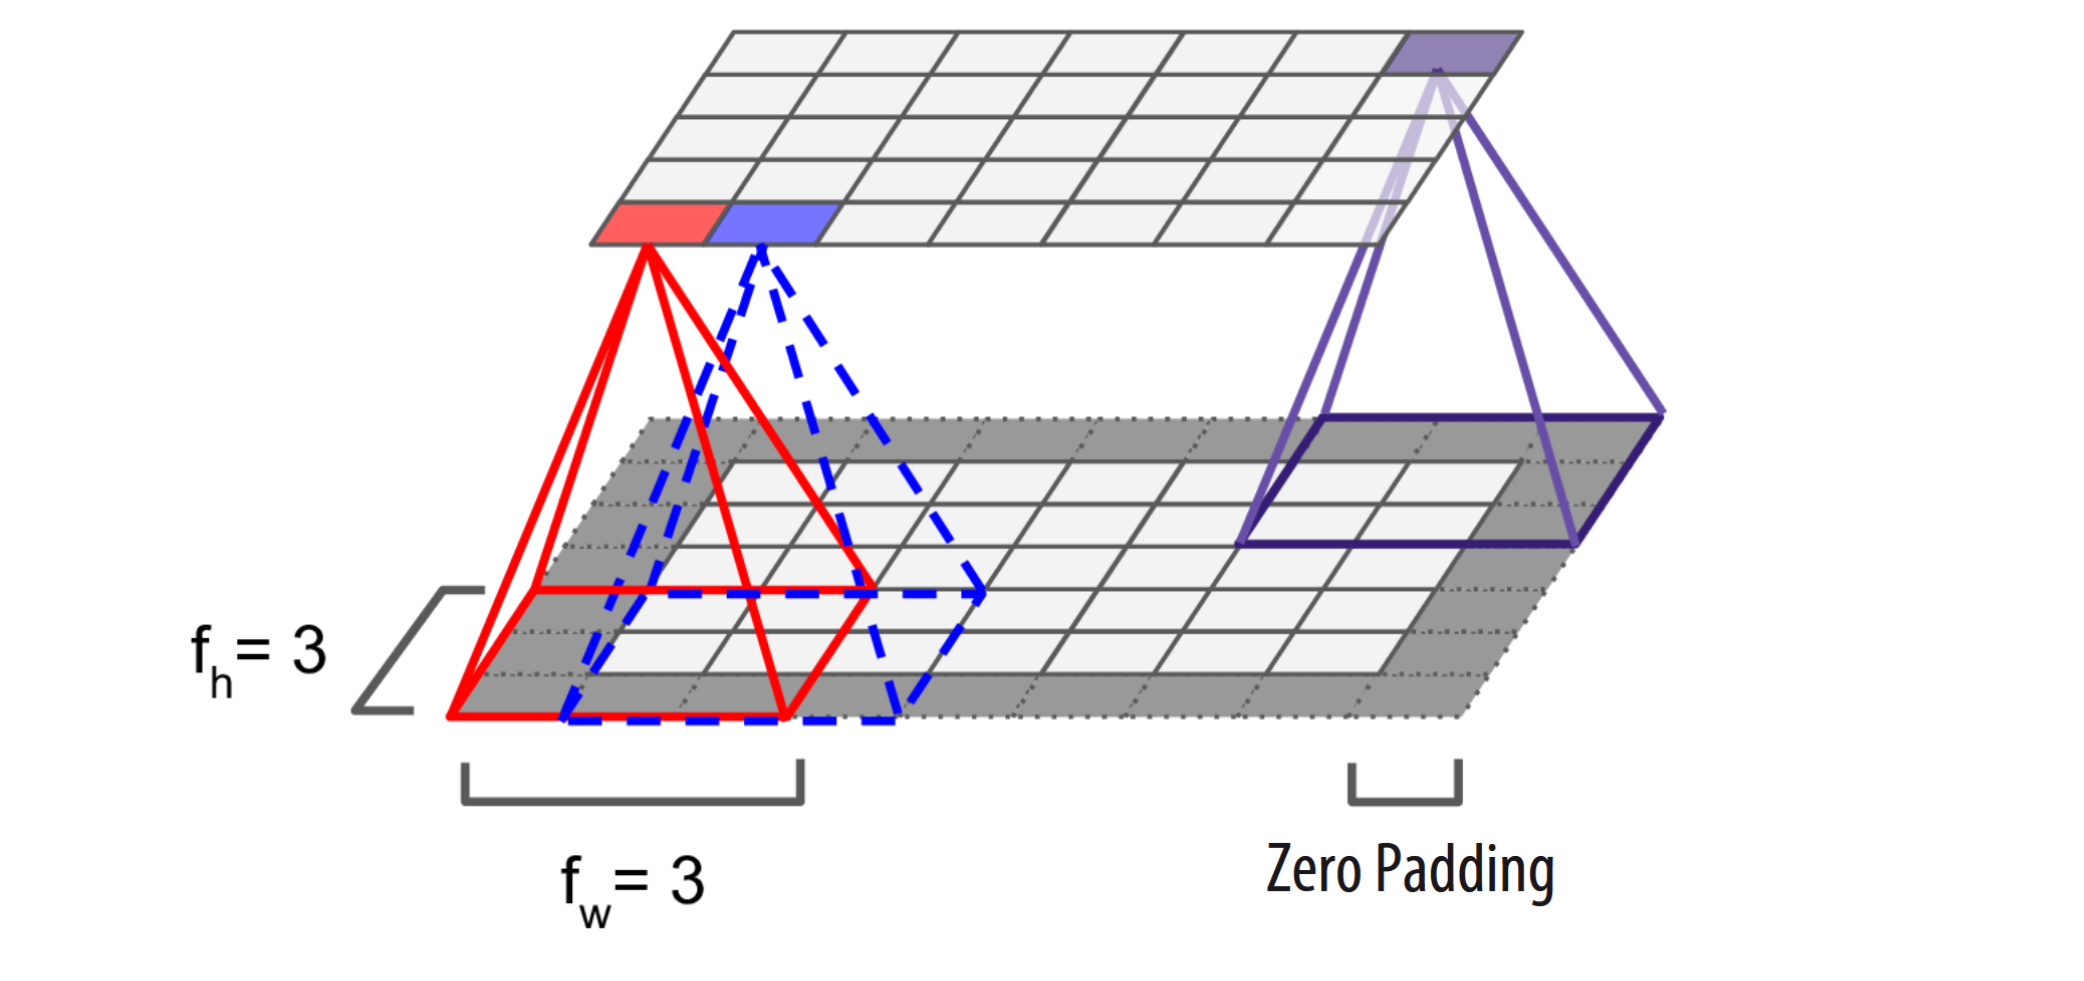
\includegraphics[width=0.85\textwidth]{cnn}
	\vspace*{-3mm}
	\caption[Einzelner Filter eines Convolutional Layers]{Ein einzelner Filter eines Convolutional Layers \cite[S.362]{MACHINE_LEARNING}.}
	\label{fig:cnn_filter}
\end{figure}
\vspace*{-5mm}
Die Arbeitsweise eines Filters ist sehr einfach zu visualisieren. Ein Filter, welcher in einer einzelnen Linie in einer vertikalen Ausrichtung hohe Gewichtungen aufweist, würde in einem Bild vertikale Linie hervorheben und horizontale Linie verschwimmen lassen. Dem gegenüber würde ein horizontaler Linienfilter, horizontale Linien hervorheben und vertikale verschwimmen lassen \cite[S.363-364]{MACHINE_LEARNING}. Ein Beispiel hierfür ist in folgender Abbildung zu erkennen:
\begin{figure}[H]
	\centering
	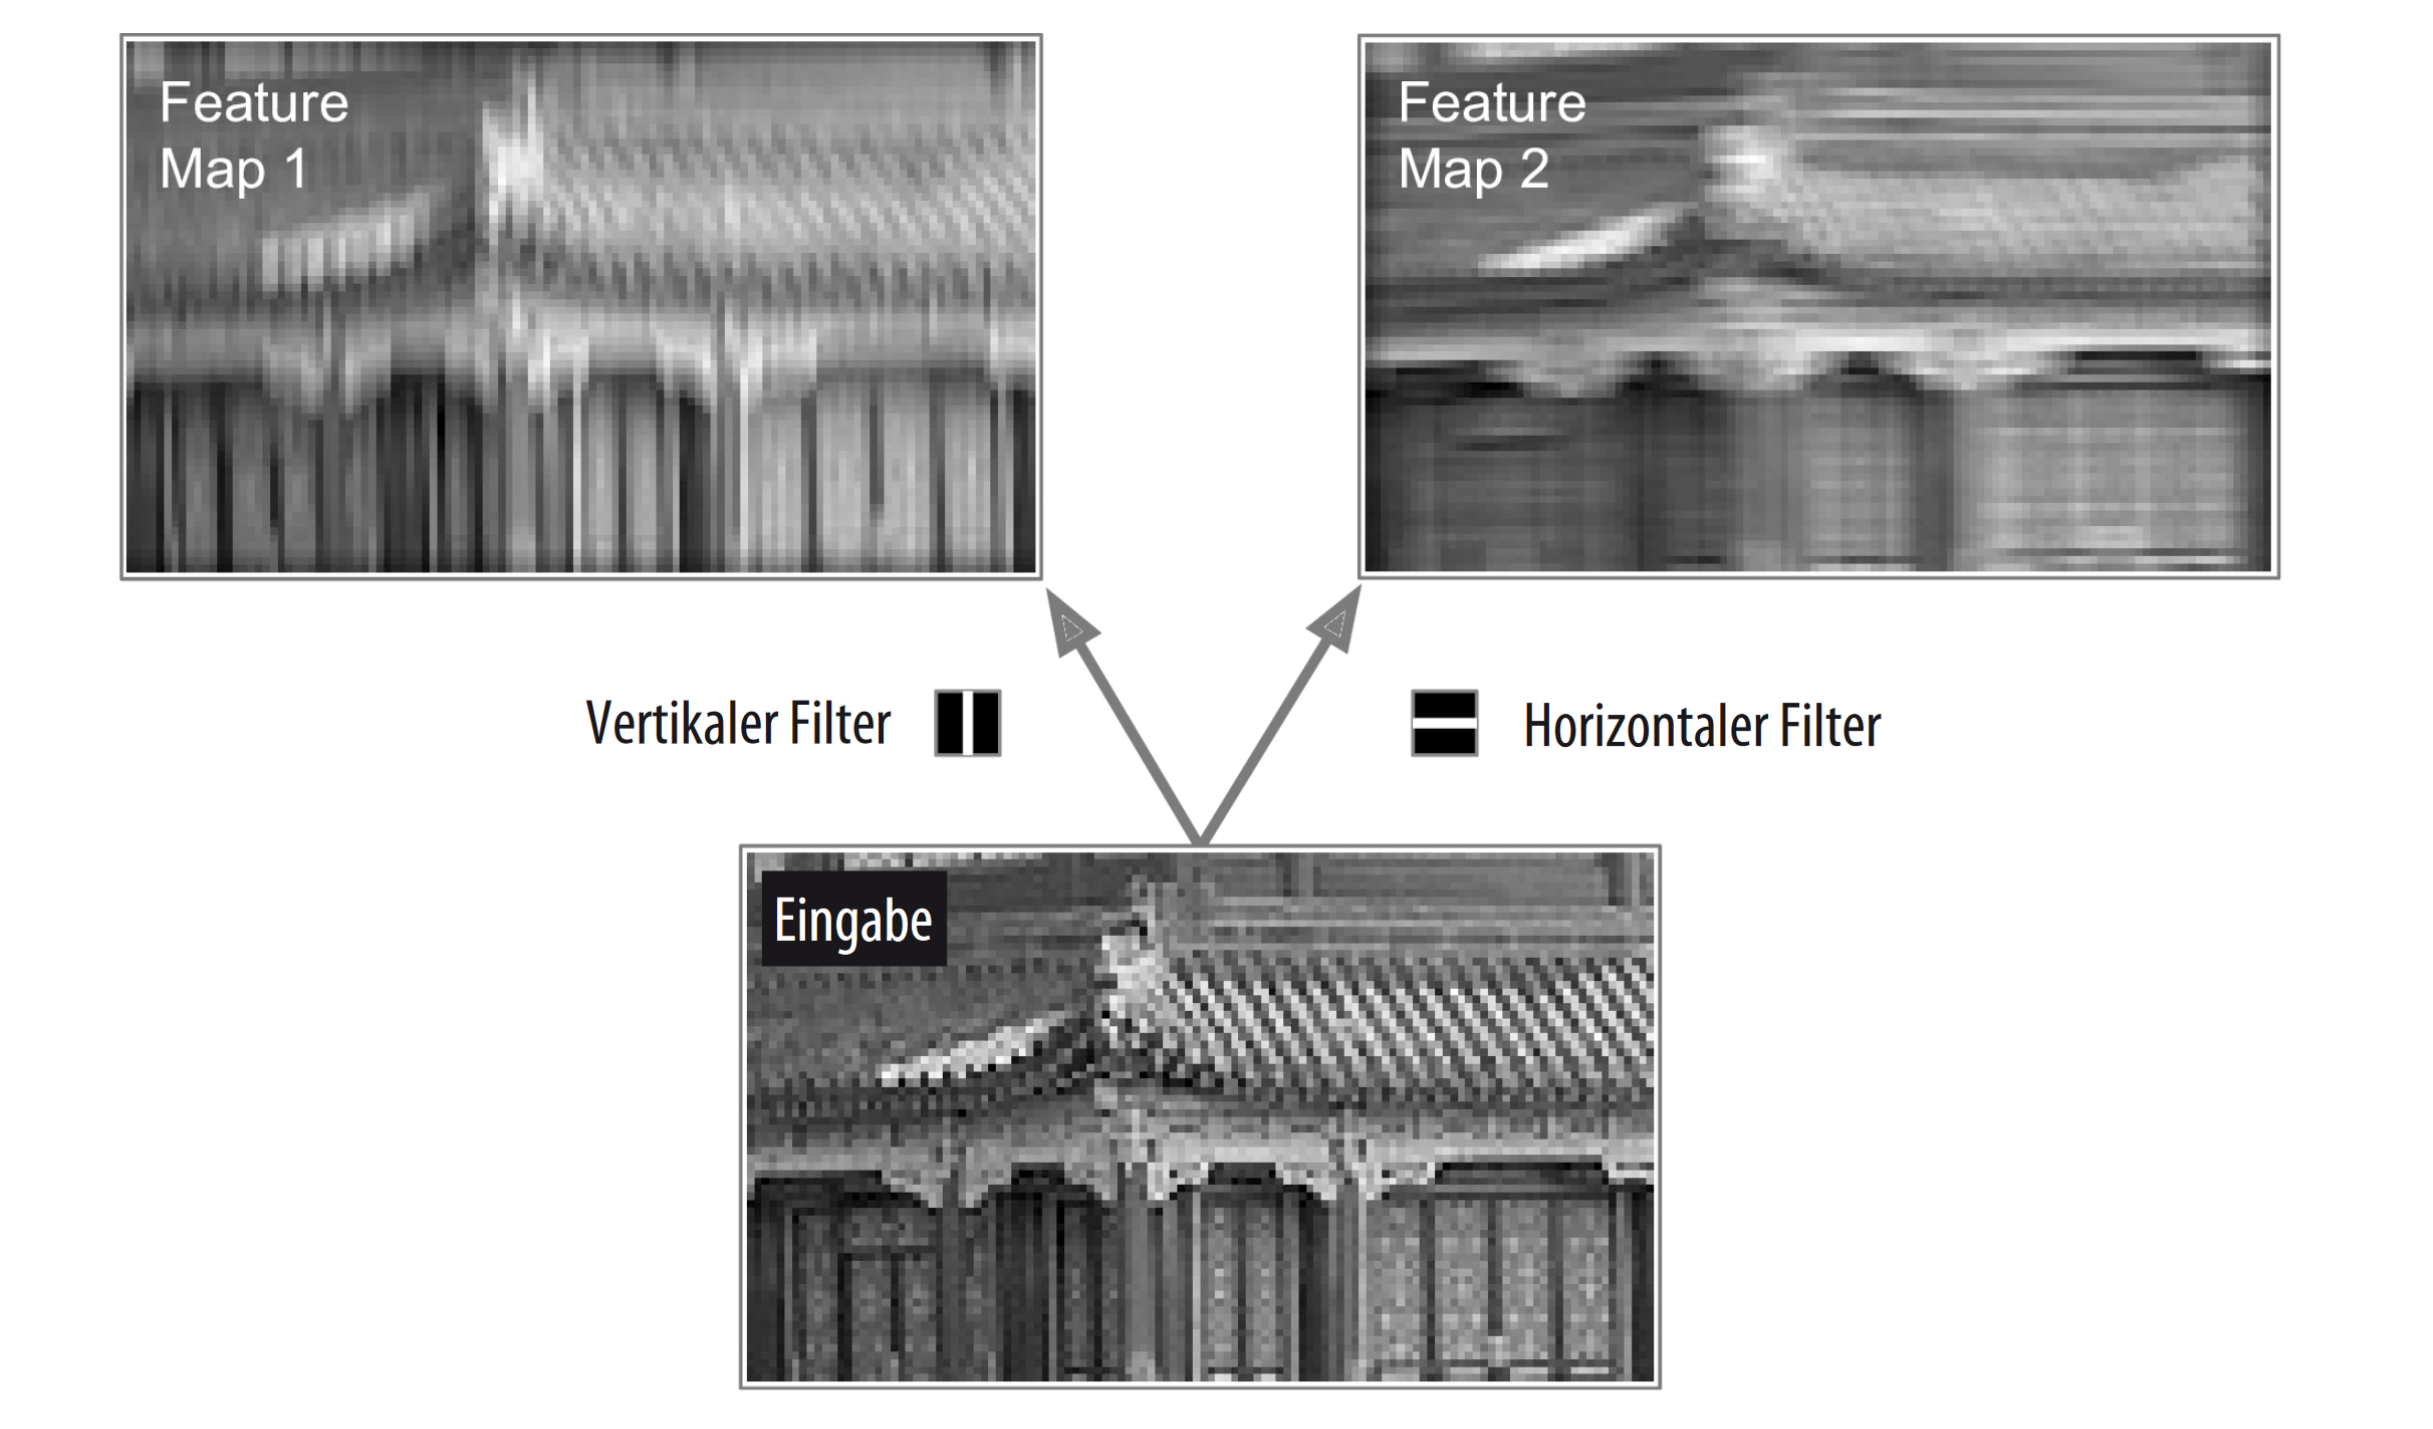
\includegraphics[width=0.85\textwidth]{filter_example}
	\vspace*{-3mm}
	\caption[Beispiel für horizontale und vertikale Filter]{Ein Beispiel für horizontale und vertikale Filter \cite[S.364]{MACHINE_LEARNING}.}
	\label{fig:cnn_filter_example}
\end{figure}
\vspace*{-5mm}
In der Abbildung \ref{fig:cnn_filter_example_2} ist außerdem ein typisches Beispiel für visualisierte Filter des ersten Convolutional Layers in einem CNN zu erkennen. Es wird klar ersichtlich, dass die dargestellten Filter verschiedene Strukturen erkennen können \cite[S.132]{DEEP_LEARNING_REVOLUTION}.
\begin{figure}[H]
	\centering
	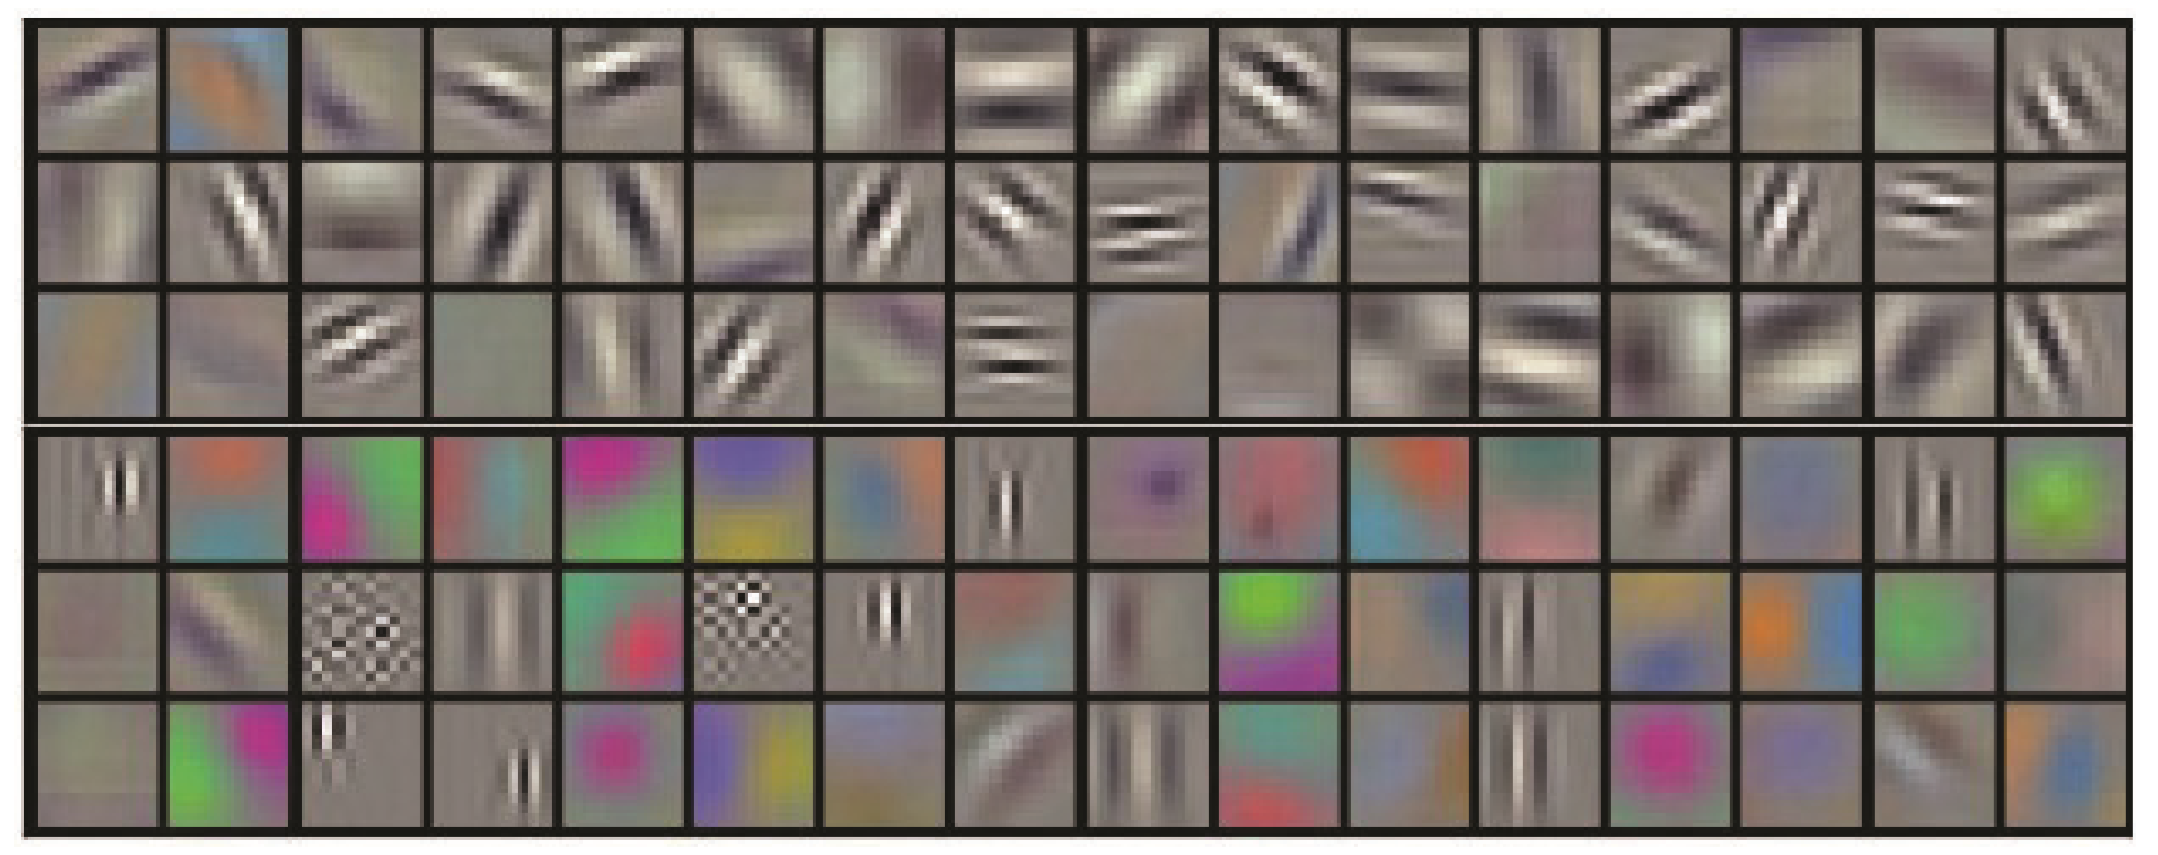
\includegraphics[width=0.85\textwidth]{cnn_filter}
	\vspace*{-3mm}
	\caption[Beispiel für verschiedene visualisierte Filter]{Ein Beispiel für verschiedene visualisierte Filter im ersten Convolutional Layers eines CNNs \cite[S.132]{DEEP_LEARNING_REVOLUTION}.}
	\label{fig:cnn_filter_example_2}
\end{figure}
\vspace*{-5mm} 
Wie in der Abbildung zu sehen, gibt es pro Convolutional Layer gleich mehrere Filter, die sogar Farben verarbeiten können. Zwar lassen sich mit mehreren bisher beschriebenen Filtern pro Convolutional Layer auch schon mehrere Features von Grauwertbildern (ein Grauwert pro Bildpunkt) sehr gut extrahieren, jedoch gehen so viele Bildinformationen der Farbe verloren, deshalb sind tatsächliche Filter in modernen CNNs eher dreidimensionale Matrizen. Die Höhe und Breite dieser ist weiterhin die selbe definierte Größe wie bei bisher bekannten Filtern, jedoch weisen sie in der Tiefe weitere Reihen von Filtern auf. Diese können Informationen aus den Farbkanälen extrahieren. Weiterhin können pro Convolutional Layer wie in der Abbildung zu sehen war, mehrere Filter eingesetzt werden. Daraus resultiert ein Stapel sogenannter Feature Maps auf denen erneut ein dreidimensionaler Filter angewandt werden kann \cite[S.364-365]{MACHINE_LEARNING}. Dies ist in folgender Abbildung gut zu erkennen:
\begin{figure}[H]
	\centering
	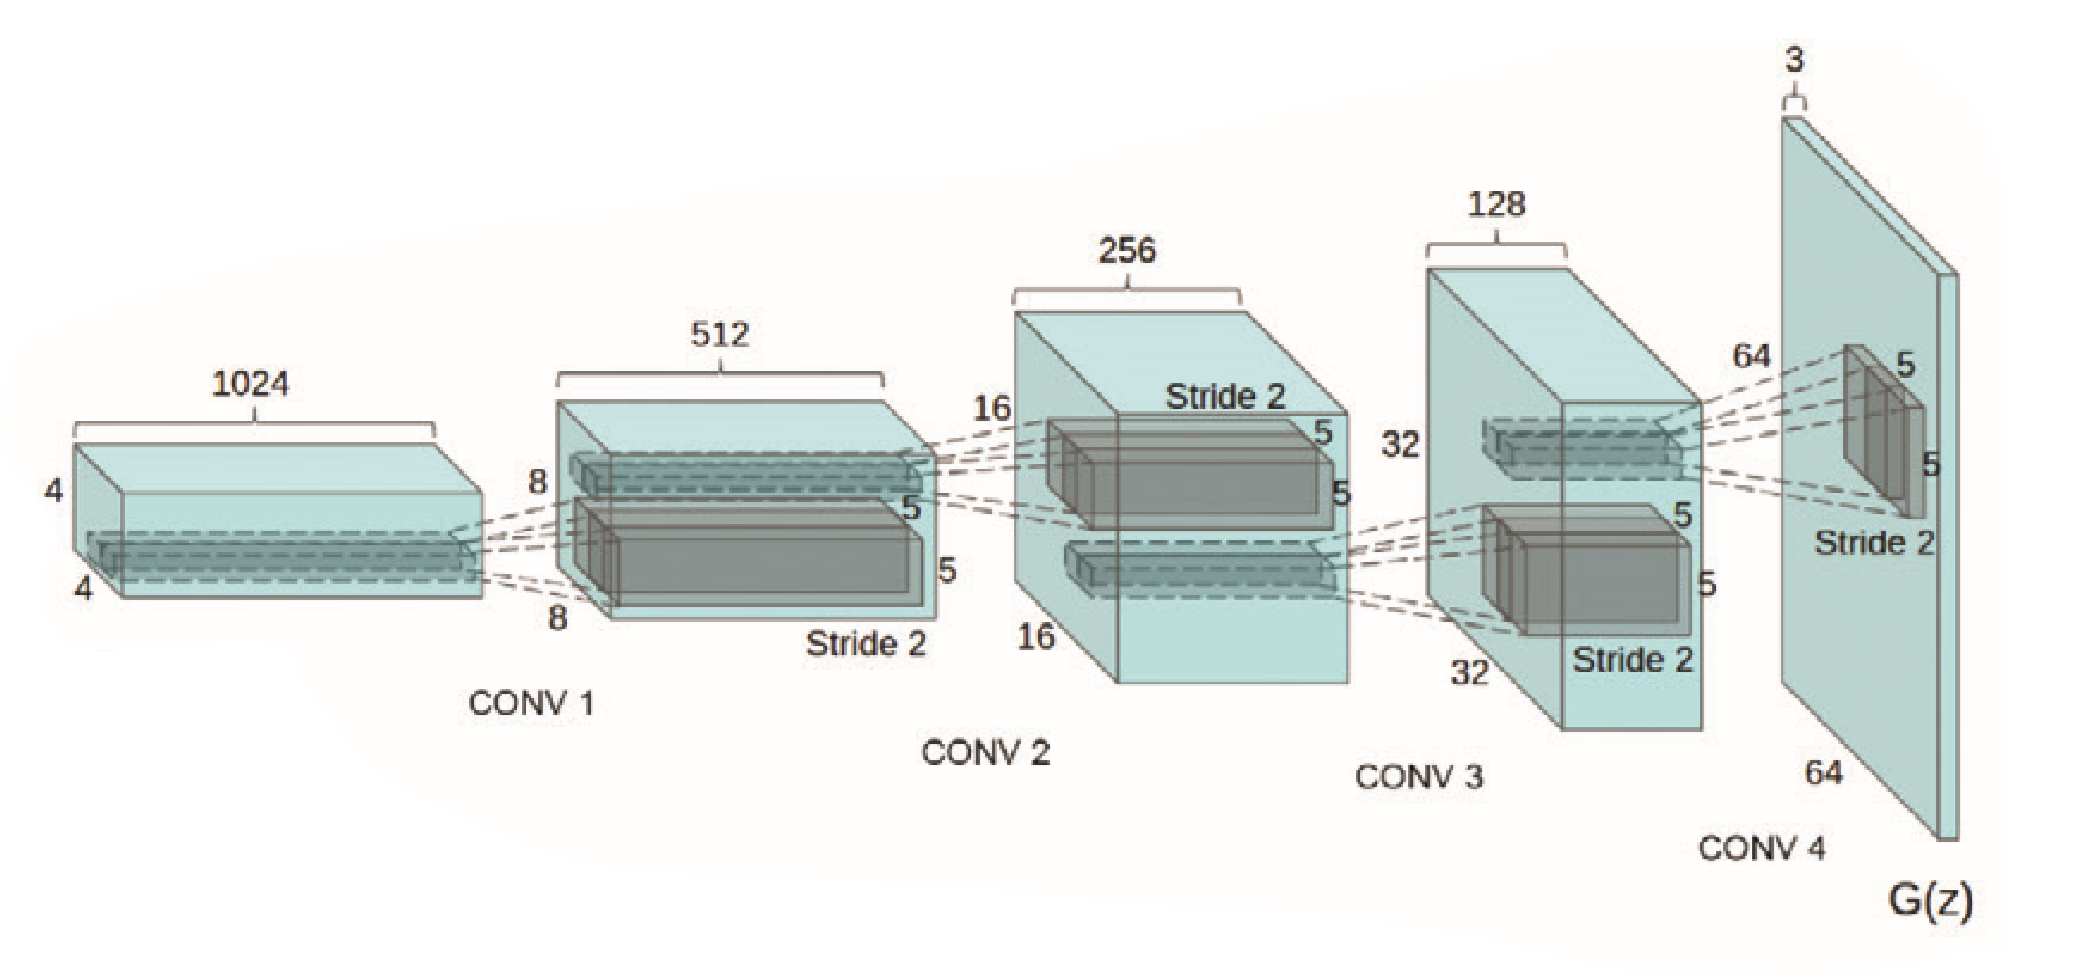
\includegraphics[width=0.85\textwidth]{cnn_3d}
	\vspace*{-3mm}
	\caption[Beispiel eines CNNs mit mehreren Feature Maps]{Ein Beispiel eines CNNs mit steigenden Feature Maps pro Layer \cite[S.138]{DEEP_LEARNING_REVOLUTION}.}
	\label{fig:cnn_3d}
\end{figure}
\vspace*{-5mm}
Die Anzahl der Feature Maps steigt in der Regel mit der Tiefe an, jedoch sollte sich ihre Größe verringern. Dies geschieht entweder über eine Schrittweite oder weiterer Methoden wie den Pooling Layern.
\subsubsection{Pooling Layer}
Pooling Layer werden genutzt um die Größe von Convolutional Layern zu verringern, indem sie zwischen diesem platziert werden und jede Feature Map oder jeden Kanal auf eine gewisse Weise verarbeiten. Die Art der Verarbeitung ist dabei abhängig vom Typ des Pooling Layers, jedoch sind Average oder Max Pooling die typischen Varianten. Beim Max Pooling wird aus einem Filter einer gewissen Höhe und Breite der Größte Wert in diesem Bereich der Feature Map entnommen. Dadurch kann dessen Größe stark verringert werden. Auch können Pooling Layer wieder eine gewisse Schrittweite (Stride) haben, mit denen die Verringerung der Größe einer Feature Map erhöht werden kann \cite[S.18-19]{DEEP_LEARNING_CV}\cite[S.369-370]{MACHINE_LEARNING}. In der Folgenden Abbildung wird die Arbeitsweise eines 2 x 2 Max Pooling mit einem Stride von 2 dargestellt: 
\begin{figure}[H]
	\centering
	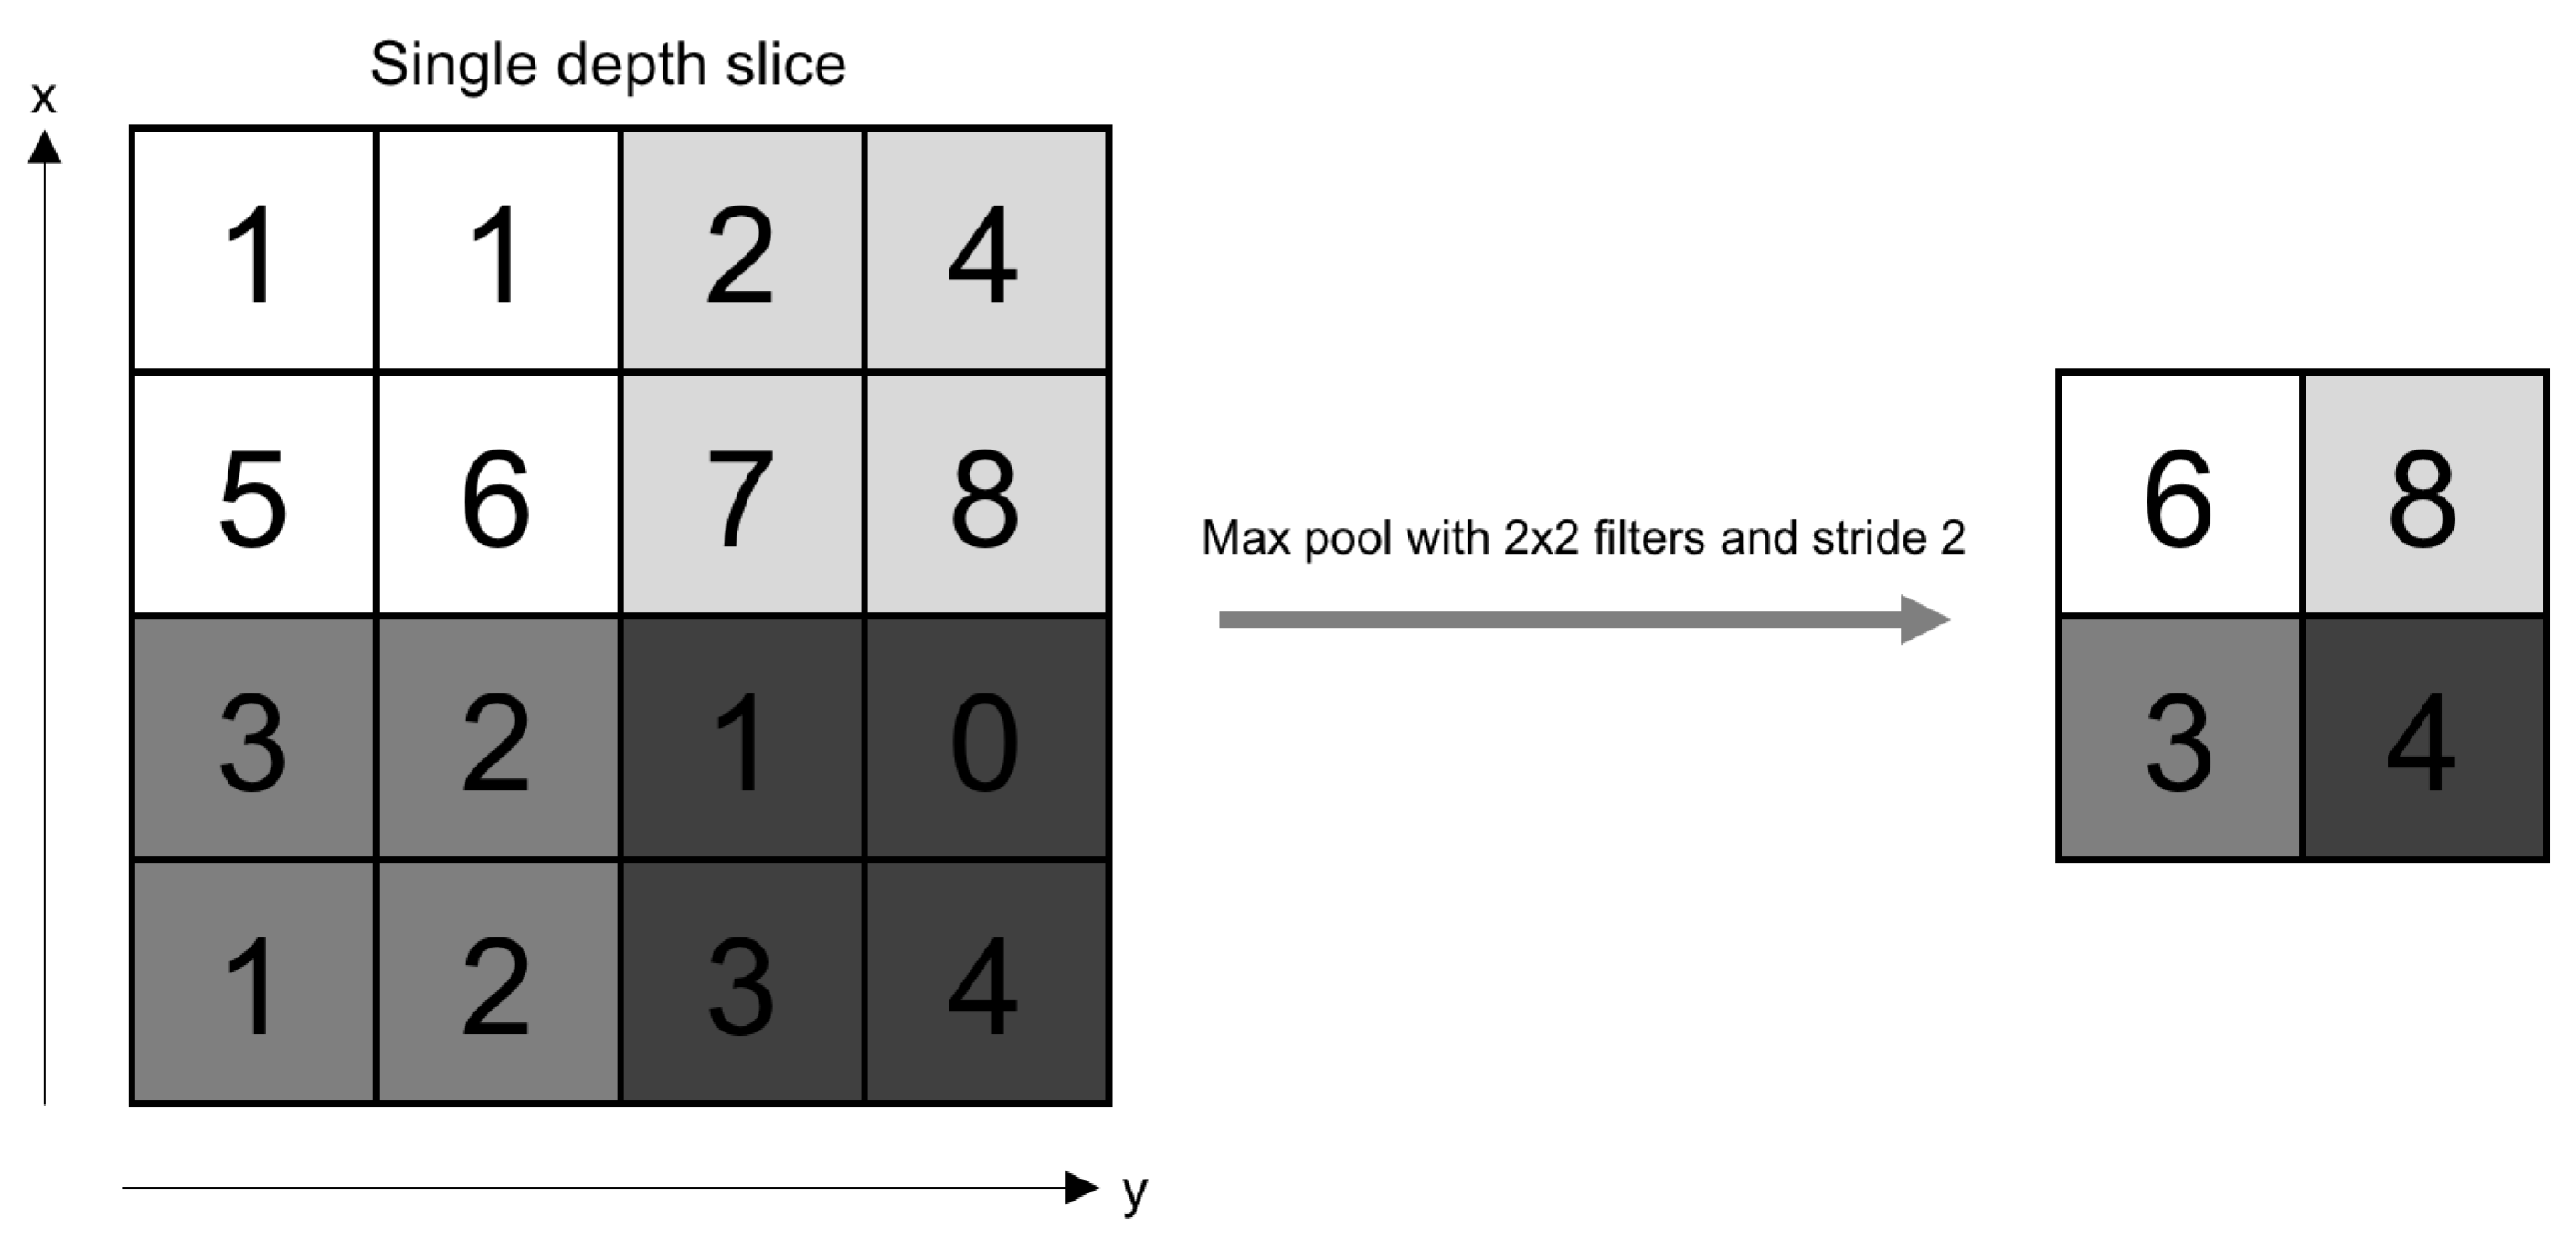
\includegraphics[width=0.85\textwidth]{pooling}
	\vspace*{-3mm}
	\caption[Arbeitsweise des Max Pooling]{Die Arbeitsweise des Max Pooling mit einem 2 x 2 Kernel und Stride von 2 \cite[S.19]{DEEP_LEARNING_CV}.}
	\label{fig:pooling}
\end{figure}
\vspace*{-5mm}
Mit der Definition der Pooling Layer sind nun die wichtigsten Grundlagen für das Maschinelle Lernen mit Bildern gesetzt. Es kann also nun mit dem praktischeren Aspekten begonnen werden.
\section{Datensätze}
\subsection{Sign Language MNIST Dataset}
\subsection{ASL Alphabet Dataset}
\subsection{Videodatensätze}
\section{Entwicklungsprozess}
Da nun die genutzten Datensätze beschrieben wurden, kann mit der Dokumentation des Entwicklungsprozesses fortgefahren werden. Hier wird wie bei Maschinellen Lernen üblich sich zunächst auf die Datenvorverarbeitung konzentriert.
\subsection{Datenvorverarbeitung}
Da die beiden hauptsächlich verwendeten Datensätze in einer für ihre Auflösung ausreichende Qualität vorhanden sind, müssen nur noch wenige Schritte in der Datenvorverarbeitung beachtet werden. Dies bezieht sich vor allem auf das Einlesen der Datensätze und das Skalieren der Bilder. Hier liefern Keras und Tensorflow in den neuesten tf-nightly Versionen (getestet mit 2.3.0a20200613) mit \lstinline[language=pythoninline]|image_dataset_from_directory| eine sehr mächtige Funktion, welche lediglich auf Basis von Ordnerstrukturen Bildatensätze mit passenden Labels erstellt und auch das Skalieren von Bildern übernehmen kann \cite{KERAS_IMAGE_PREPROCESSING}. Dabei wird beim Aufruf ein Tensorflow Dataset zurückgegeben, das bereits Pipelining einer gewissen Batchgröße von der Festplatte unterstützt. Dies ist bei sehr großen Datensätzen nützlich. Nun, müssen die Datensätze lediglich in passenden Ordnerstrukturen umgewandelt werden, bei denen alle Bilder einer Klasse einen Ordner mit passender Bezeichnung nutzen. Außerdem ist eine Teilung in Test, sowie Trainings- und Validierungsdaten nötig, denn \lstinline[language=pythoninline]|image_dataset_from_directory| unterstützt lediglich eine Zweiteilung. 
\subsubsection{Sign Language MNIST Dataset}
Dieser Datensatz besteht im Kern aus zwei CSV Dateien für Training- und Test. Die Zeilen repräsentieren dabei die 28x28 Pixel eines Grauwertbildes, sowie ein Label in der ersten Spalte. Die Label sind Zahlen von 0-25 und repräsentieren alle Buchstaben des Alphabets außer Z (25) und J (9), welche ausgelassen wurden. Trotz des Aufbaus in CSV Dateien, wurde sich entschieden die Werte zu extrahieren und als einzelne PNGs in die erforderlichen Ordnerstrukturen abzuspeichern. Der Kern der Skriptdatei zur Vorverarbeitung des Sign Language MNIST Dataset ist dabei folgende Funktion:
\begin{lstlisting}[language=python,firstnumber=36,caption={Kern der Sign Language MNIST Dataset Vorverarbeitung.},label=lst:to_image_at_dir]
def to_image_at_dir(target_dir, row_data, image_name):
	"""
	Wandelt die Zeilen einer CSV Datei im Datensatz in ein Bild um.
	:param target_dir: Zielordner
	:param row_data: Daten der Zeile.
	:param image_name: Name des Bildes.
	:return: None.
	"""
	# Label entnehmen.
	label = row_data[0]
	# Daten entnehmen in Integer umwandeln.
	list_data = list(map(int, row_data[1::]))
	
	# Image Data in Numpy 28x28 Array umwandeln.
	image_data = numpy.reshape(numpy.array(
	list_data, dtype=numpy.uint8), (28, 28))
	label_folder = target_dir + str(label) + "/"
	
	# Ordner erstellen, wenn nicht vorhanden.
	os.makedirs(label_folder, exist_ok=True)
	# Bild erstellen.
	image = Image.fromarray(image_data)
	# Bild als PNG speichern.
	image.convert("RGB").save(label_folder + image_name + ".png")
\end{lstlisting}
Diese Funktion ist sehr einfach und nimmt lediglich einen Zielordner, die Daten einer Zeile des Datensatzes sowie ein Name des Bildes (zum Beispiel eine Bildnummer) an. Dann werden in Zeile 45 und 47 Label und Daten getrennt. Eine Umwandlung in Integer der Daten wird ebenfalls über eine Map-Funtkion vorgenommen. Es folgt in Zeile 50 bis 52 eine Umwandlung in ein 28x28 Numpy-Array mit Datenpunkten als 8-Bit Unsigned Integer (uint8). Zuletzt werden die Daten des Numpy-Arrays lediglich mit der bekannten Bildverarbeitungsbibliothek für Python Pillow in ein Bild umgewandelt und anschließend als PNG in RGB abgespeichert. Es wurde sich hier für PNGs statt für Grauwertbilder entschieden, da so ein problemloses Verwenden von \lstinline[language=pythoninline]|image_dataset_from_directory| möglich wird.
\subsubsection{ASL Alphabet Dataset}
Der ASL Alphabet Dataset ist vom Aufbau deutlich einfacher zu verarbeiten, da hier die Bilder bereits in passende Subordner des Trainingsdatensatzes sortiert sind. Die Testdaten benötigen allerdings Vorverarbeitung, da diese pro Zeichen der ASL nur ein Bild beinhalten. Dies ist nicht hinreichend für Testdaten. In der Vorverarbeitung wird also eine bestimmte Anzahl zufälliger Bilder pro ASL Zeichen aus den Trainingsdaten ausgewählt und in das passend erstellte Verzeichnis für die Testdaten umkopiert.
\\\\
Dies funktioniert im Kern über folgende Funktion, welche jeden Ordner für ein ASL Zeichen durchläuft und mittels der Bibliothek \lstinline[language=pythoninline]|glob| alle Dateien aus diesen ließt. Dann werden mit \lstinline[language=pythoninline]|random.sample| eine vorher definierte zufällige Anzahl von Samples (in der Praxis 300) ausgewählt und in das Zielverzeichnis des Testordners für dieses ASL Zeichen umkopiert.
\begin{lstlisting}[language=python,firstnumber=44,caption={Kern der Sign Language MNIST Dataset Vorverarbeitung.},label=lst:to_image_at_dir]
# Bewege die in rand_num_to_move definierte Anzahl 
# zufälliger Elemente pro Klasse in den Testordner.
for target_dir_name in glob.glob(target_directory + "/" + 
		train_directory_name + "/*"):
	
	target_dir_classes = glob.glob(target_dir_name + "/*")
	# Wähle für diese Klasse rand_num_to_move zufällige Elemente aus.
	random_elements = random.sample(target_dir_classes, 
		rand_num_to_move)
	# Kopiere die Elemente um.
	for move_element in random_elements:
		new_dir = move_element.replace(train_directory_name, 
			test_directory_name)
		os.makedirs(os.path.dirname(new_dir), exist_ok=True)
		shutil.move(move_element, new_dir)
\end{lstlisting}
\subsubsection{DatasetParser Pakete}
Das Ziel der DatasetParser Python Pakete ist es, für alle vorverarbeiteten Datensätze eine vereinigte Schnittstelle zum Bereitstellen von Datensätzen zu liefern. Diese bestehen aus einer DatasetParser Datei mit den Funktionen \lstinline[language=pythoninline]|get_train_and_val| und \lstinline[language=pythoninline]|get_test|, welche Trainings-, Test- und Validierungsdaten bereitstellen, sowie den Konstanten \lstinline[language=pythoninline]|class_names| und \lstinline[language=pythoninline]|image_size|, die Klassennamen (im Bezug auf die Ordner der vorverarbeiteten Datensätze) und eine standardmäßige Bildgröße definieren. Eine weitere in den Paketen nötige Skriptdatei ist DatasetPrepareOrig. Diese führt mittels einer separaten Ausführung eine in den vorherigen Kapiteln beschriebene Vorverarbeitung aus. Der Datensatz selber ist nun in DatasetOrig, als nicht verarbeiteter Datensatz, und in DatasetPrepared, als durch das Skript vorverarbeiteter Datensatz, definiert.
\\\\
Die Arbeitsweise der DatasetParser Dateien ist nun sehr einfach zu beschreiben. Diese führen beim Aufruf von \lstinline[language=pythoninline]|get_train_and_val| zweimal die Tensorflow-Funktion \lstinline[language=pythoninline]|image_dataset_from_directory| mit vom Datensatz abhängigen Parametern auf und geben die Ergebnisse dieser zurück. Wird unter der Angabe des Parameters \lstinline[language=pythoninline]|validation_split| diese Funktion auf ein Verzeichnis zweimal ausgeführt, so gibt Tensorflow beim ersten Aufruf das Dataset der Trainings- und beim zweiten das Dataset der Validierungsdaten zurück. Die Testdaten der Funktion \lstinline[language=pythoninline]|get_test| werden über einen einzelnen Aufruf ohne \lstinline[language=pythoninline]|validation_split| zurückgegeben.
\begin{lstlisting}[language=python,firstnumber=1,caption={Beispielhafter Aufruf der Funktion zum Einlesen von Daten},label=lst:dataset]
return image_dataset_from_directory(
	directory="datasets/kaggle_1/DatasetPrepared/train",
	label_mode='categorical',
	color_mode='grayscale',
	image_size=image_size_param,
	batch_size=batch_size,
	shuffle=shuffle,
	seed=seed,
	validation_split=validation_split,
	subset="training",
	interpolation='bilinear',
	follow_links=False
)
\end{lstlisting}
Im Listing \ref{lst:dataset} wird ein Aufruf der Funktion \lstinline[language=pythoninline]|image_dataset_from_directory| beschrieben. Die wichtigsten Parameter haben dabei folgende Aufgaben:
\begin{itemize}
	\item \lstinline[language=pythoninline]|directory|: Das Verzeichnis aus dem der Datensatz gelesen wird.
	\item \lstinline[language=pythoninline]|label_mode|: Bei categorical werden die Subordner als Kategorien gesehen und als One-Hot kodierten Vektor beschrieben.
	\item \lstinline[language=pythoninline]|color_mode|: Umgewandelte Farbkanäle der Bilder.
	\item \lstinline[language=pythoninline]|image_size|: Skalierte Größe der Bilder.
	\item \lstinline[language=pythoninline]|batch_size|: Größe der Batches des Datasets.
	\item \lstinline[language=pythoninline]|shuffle|: Werden die Bilder nach dem Einlesen zufällig angeordnet.
	\item \lstinline[language=pythoninline]|validation_split|: Anteil der Validierungsdaten.
	\item \lstinline[language=pythoninline]|subset|: Das zurückgegebene Subset für dieses Verzeichnis. Dieses ist entweder training oder validation.
	\item \lstinline[language=pythoninline]|interpolation|: Genutztes Verfahren für die Skalierung.
\end{itemize}
Da die Datensätze für ihre Auflösung alle eine sehr rauschfreies Bild aufweisen und in der Regel schon recht gut auf die Hände fokussiert sind, ist damit nun die Datenvorverarbeitung abgeschlossen und die Bilder der Datensätze können sehr einfach in passende Tensorflow-Datasets gelesen werden. Nun, wird die Entwicklung und Auswertung von Modellen beschrieben.
\subsection{Entwickelte Modelle}
In diesem Kapitel wir der Grundaufbau der Python-Dateien zum Maschinellen Lernen vorgestellt und die Ergebnisse einiger Modelle vorgestellt. Dabei werden für Neuronale Netze, Konvolutionelle Neuronale Netze und Transferlearning einige der besten Versuche vorgestellt. 
\subsubsection{Grundaufbau des Modelltrainings}
Alle Dateien für das Training von Modellen haben grundsätzlich einen ähnlichen Aufbau. Zunächst müssen die DatasetParser der gewünschten Datensätze inkludiert werden mit welchen ein Großteil der Datenvorverarbeitung schon erledigt werden kann. Danach folgen in der Regel einige Definitionen für Batchgröße und Bildgröße, mit welchen nun die Funktionen \lstinline[language=pythoninline]|get_train_and_val| und \lstinline[language=pythoninline]|get_test| aufgerufen werden können. Dank sinnvoller Default-Parameter ist dieser Aufruf in der Regel recht kurz. Es wurde ein 80-20 Validation Split unter einer in Kapitel \ref{validation} beschriebenen Validierung in drei Stufen verwendet. Am Ende der Vorbereitung wird in der Regel noch die Anzahl der Klassen für die Ausgabe und die Größe der Eingabe für den ersten Layer des Modells definiert. Ein Beispiel für die Vorbereitung des Trainings ist im folgenden Listing zu erkennen:
\begin{lstlisting}[language=python,firstnumber=1,caption={Beispielhafte Vorbereitung für das Training},label=lst:pre_train]
from sign_language_image.datasets.kaggle_1.DatasetParser
	import get_train_and_val, get_test, class_names 
...
# Batchgröße
batch_size = 100
# Bildgröße
image_size = (28, 28)
train_ds, val_ds = get_train_and_val(batch_size, 
	image_size_param=image_size)
test_ds = get_test(image_size_param=image_size)

# Anzahl der Klassen aus den Namen der Klassen extrahieren
num_of_classes = len(class_names)
# Input Shape als Bildgröße + Farbkanäle
input_shape = (image_size[0], image_size[1], 1)
\end{lstlisting}
Danach kann dann schon ein Modell definiert werden. Diese können sich je nach Aufbau etwas unterscheiden, daher wird auf sie und ihre Ergebnisse in den nächsten Kapiteln eingegangen.
\\\\
Nach der Definition eines Modells kann dieses kompiliert und mit einem Optimizer und Qualitätsmaß versehen werden. Hier wurde aufgrund des Aufbaus der Daten und des Lernziels die Kreuzentropie genutzt. Außerdem wird ein Modell während der Optimierung über die Vorhersagegenauigkeit auf Trainings- und Validierungsdaten ausgewertet. Dies ist aufgrund der gleichmäßigen Verteilung und Priorität der Klassen in den Datensätzen möglich. Als Optimierer wird eine Erweiterung des stochastische Gradientenverfahren den Adam-Optimierer genutzt.
\begin{lstlisting}[language=python,firstnumber=1,caption={Kompilierung eines Modells},label=lst:compile_model]
# Modell kompilieren mit Kreuzentropie und Adam Optimizer.
model.compile(loss='categorical_crossentropy',
	optimizer=tf.keras.optimizers.Adam(lr=0.00005),
	metrics=['accuracy'])
\end{lstlisting}
Dann wurde eine Funktion für das Loggen entwickelt. Diese kopiert das momentan aktive Skript in einen eigenen Ordner eines übergebenen Logverzeichnisses. Dieses dient als Referenz, wenn die originale Trainingsdatei verändert wurde. Dann wird abhängig von einem Parameter die Ausgabe der Konsole in eine Logdatei in dem vorher erstellten Verzeichnis umgeleitet, um später den Trainingsvorgang nachvollziehen zu können. Zuletzt werden zwei Tensorflow-Callbacks für das Verzeichnis erstellt, welche TensorBoard-Logs erstellen und die Modelle mit dem geringsten Fehler abspeichern.
\begin{lstlisting}[language=python,firstnumber=1,caption={Logging Funktion für Trainingsvorgänge},label=lst:log_train]
def log_run(log_dir, log_to_file=True):
	script_path = sys.argv[0]
	script_name = os.path.basename(script_path)
	log_dir_script = log_dir + script_name + "_" + 	 datetime.now().strftime("%d-%m-%Y_%H%M%S") + "/"
	# Erstelle das Log Verzeichnis
	os.makedirs(log_dir_script)
	# Kopiere das Script, welches ausgeführt wurde in das Log Verzeichnis
	shutil.copy(script_path, log_dir_script + script_name)
	# Leite Ausgabe der Konsole um
	if log_to_file:
		print("Starting Log To File!")
		sys.stdout = open(log_dir_script + script_name + 
			".log.txt", "w")
	
	# Erstelle und gebe Callbacks für das Log-Verzeichnis zurück.
	return tf.keras.callbacks.TensorBoard(
		log_dir=log_dir_script, profile_batch=5), \
		tf.keras.callbacks.ModelCheckpoint(log_dir_script + 'model.mdl_wts.hdf5', save_best_only=True,
		monitor='val_loss', mode='min'), log_dir_script
\end{lstlisting}
Im Folgenden wird lediglich nur noch ein Callback eingeführt, welches das Training nach einer gewissen Zahl von Durchläufe in welchen sich der Fehler des Modells nicht verbessert abbricht. Dann kann das Modell mit Trainingsdaten und Validierungsdaten zur Überprüfung folgendermaßen für eine maximale Anzahl von Epochen antrainiert werden:
\begin{lstlisting}[language=python,firstnumber=1,caption={Start des Trainings mit Keras},label=lst:train_start]
model.fit(train_ds,
	epochs=50,
	verbose=1,
	validation_data=val_ds,
	callbacks=[tensorboard_callback, checkpoint, es])
\end{lstlisting}
Nach dem Trainingsvorgang wird nun die beste Epoche aus dem Logverzeichnis geladen und mit den Testdaten überprüft. Dann wird zunächst die \lstinline[language=pythoninline]|evaluate| Methode des Keras-Modells genutzt, um eine Vorhersagegenauigkeit und den Fehler auf den Testdaten zu bestimmen. Zum Schluss wird mittels Scikit-Learn in der eigens definierte \lstinline[language=pythoninline]|evaluate| Funktion eine Konfusionsmatrize und Auswertungstabelle mit Precision, Recall und F1-Score zu den Testdaten erstellt. Dies ist im folgenden Listing erkennbar:
\begin{lstlisting}[language=python,firstnumber=1,caption={Auswertung eines Modells mit Testdaten},label=lst:modell_eval]
# Lade das beste Modell
model = load_model(run_path + "model.mdl_wts.hdf5")
# Score auf den Testdaten
score = model.evaluate(test_ds, verbose=1)
print('Test loss:', score[0])
print('Test accuracy:', score[1])

# Entnehme aus dem Test Datensatz, zur Anwendung mit sklearn
test_data_labels = []
for data, label in test_ds.take(-1):
	test_data_labels.extend(label)

# Prediction für den Test Datensatz
pred = model.predict(test_ds, verbose=1)
# Evaluiere die Ergebnisse vom Testdatensatz mit sklearn
evaluate(numpy.argmax(pred, axis=1), 
	numpy.argmax(test_data_labels, axis=1))
\end{lstlisting}
Abschließend sei erwähnt, dass die Auswertungsergebnisse der Testdaten nur in Betracht gezogen wurden, wenn bereits einige andere Modelle mit Validierungsdaten getestet wurden. Ein anderes Auswertungsverhalten würde die in Kapitel \ref{validation} genannten Grundsätze verletzen.
\subsubsection{Neuronale Netze}
Zunächst wurde der Einsatz einfacher Neuronaler Netze erprobt. Da diese grade bei großen Bildern in der Regel von CNNs abgelöst wurden, wurden hier nur wenige Tests ausgeführt. Selbst bei großen Modellen und ohne vorliegenden Overfitting Effekten, konnte maximal eine Vorhersagegenauigkeit von 80\% erreicht werden. Eines dieser Modelle, welches für das Sign Language MNIST Dataset verwendet wurde, ist in folgender Abbildung zu erkennen: 
\begin{figure}[H]
	\centering
	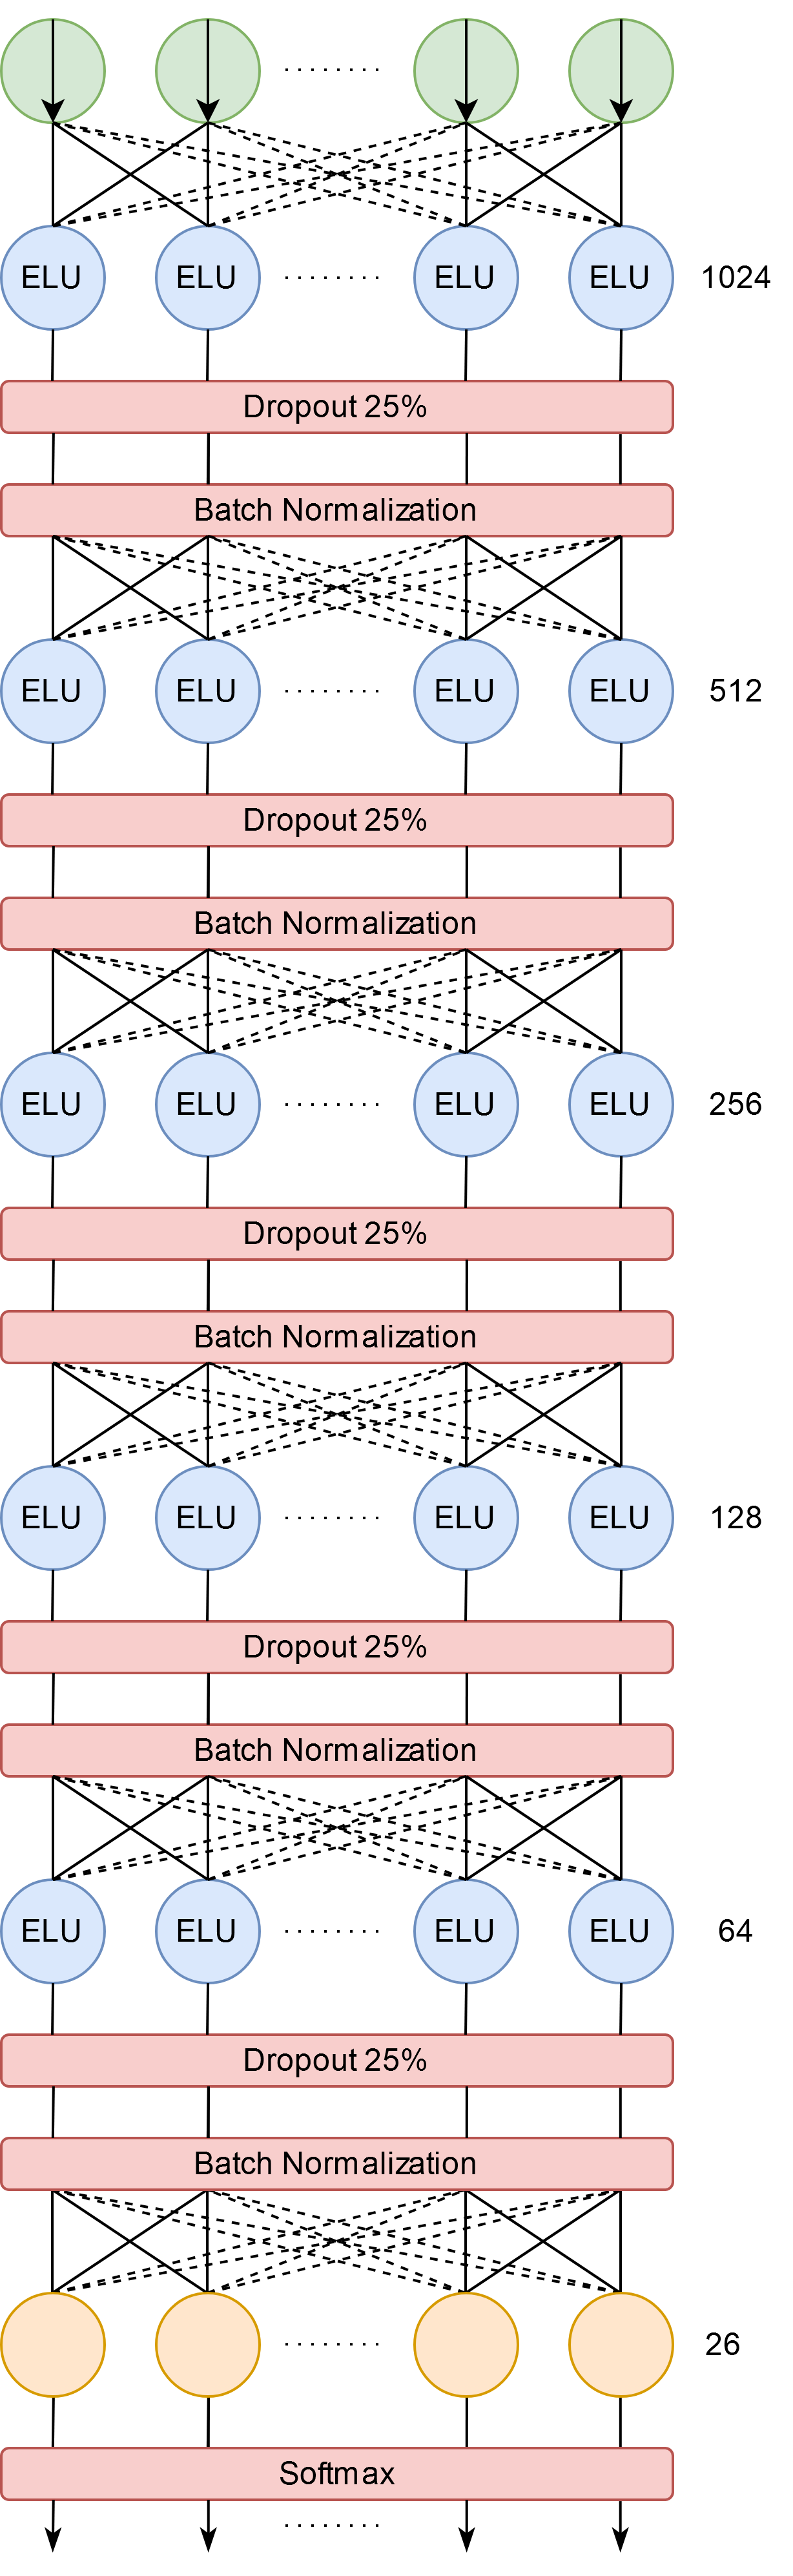
\includegraphics[width=0.50\textwidth]{nn_1}
	\vspace*{-3mm}
	\caption[Eingesetztes Neuronales Netz mit fünf Hidden-Layern]{Ein eingesetztes Neuronales Netz mit fünf Hidden-Layern.}
	\label{fig:nn_1}
\end{figure}
\vspace*{-5mm}
Dieser erreicht auf dem genutzten Datensatz lediglich eine Vorhersagegenauigkeit von 78\% auf den Validierungsdaten. Auf den Testdaten erreicht dieses Modell 81\% Vorhersagegenauigkeit und F1-Score. Dies ist zwar etwas besser, jedoch nicht in einem gewünschten Bereich.
\\\\
Mit dem ASL-Alphabet Dataset gibt es noch größere Probleme im Einsatz normaler Neuronaler Netze. Die Bilder weisen alle eine Größe von 200x200 Pixeln auf, was in einer Eingabegröße von 40000 Pixeln mit drei Kanälen resultieren würde. Die eingegebenen Bilder werden beim Einlesen daher auf 50x50 Grauwerte reduziert. Selbst damit wurde ein siebter Layer mit 2048 ELU-Neuronen an den Anfang des Netzes eingeführt werden, um die 2500 Eingabewerte sinnvoll aufnehmen zu können.
\subsubsection{Konvolutionelle Neuronale Netze}
\subsubsection{Transfer Learning mittels VGG19}
Bei vielen Problemen des maschinellen Lernens, ist es sinnvoll ganze oder Teile von vortrainierten Modellen zu verwenden. Dies ist besonders bei vielen Bereichen der Bilderkennung sinnvoll und üblich. Die Wiederverwendung von Modellen wird auch als Transfer Learning bezeichnet \cite[S.287]{MACHINE_LEARNING}. Ein solches Modell soll nun auch in diesem Projekt angewandt werden. Es wurde sich für das VGG19 entschieden, da dieses laut der basierenden Arbeit eine sehr gute Generalisierung für andere Datensätze besitzt und von Keras unterstützt wird \cite{VGG19}. Es ist folgendermaßen aufgebaut:
\begin{figure}[H]
	\centering
	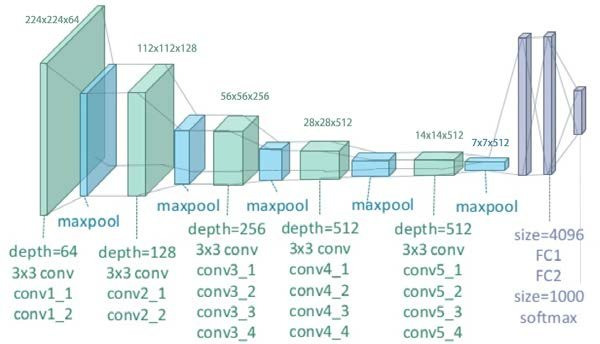
\includegraphics[width=0.80\textwidth]{vgg_19_img}
	\vspace*{-3mm}
	\caption[Aufbau des VGG19]{Der Aufbau des VGG19 \cite{VGG_19_IMG}.}
	\label{fig:vgg_19}
\end{figure}
\vspace*{-5mm}
Es ist zu beachten, dass sich Filter der selben Größe mehrfach wiederholen, sodass mit den vollständig verbundenen Schichten ein Konvolutionelles Neuronales Netz mit 19 Layern entsteht. Die vollständig verbundenen Schichten können in Keras ausgeschaltet werden, was in diesem Fall des Transfer Learning aufgrund der unterschiedlichen Zahl von nützlichen Ausgabeneuronen (das Netz sieht 1000 vor) sinnvoll ist. 
\subsection{Backend der Webanwendung}
\subsection{Frontend der Webanwendung}
\subsection{Ergebnisse der Entwicklung}
\section{Fazit} 
\section{Ausblick}
\setcounter{biburllcpenalty}{7000}
\setcounter{biburlucpenalty}{8000}
\pagebreak
\printbibliography[title=Quellen]
\end{document}